\graphicspath{{chapt_dutch/}{intro/}{chapt2/}{chapt3/}{chapt4/}{chapt5/}{chapt6/}{chapt7/}{chapt8/}}

% Header
\renewcommand\evenpagerightmark{{\scshape\small Chapter 2}}
\renewcommand\oddpageleftmark{{\scshape\small The Standard Model and Beyond}}

\renewcommand{\bibname}{References}

\hyphenation{}

\chapter[The Standard Model and Beyond]%
{The Standard Model and Beyond}\label{chapt:3}
\section*{Introduction}
This chapter describes the Standard Model (SM) of particle physics, the physics of top quark and the SM higgs boson, the most important constituents of the SM. The discussion follows introduction to the extensions the SM (SUSY), higgs searches using different models and CMS searches in BSM area. The last part is devoted to the search of the neutral heavy higgs decays into two a pair of ($H \rightarrow t\bar{t}$) using the resonance and interference phenomena.    
\section{The Standard Model}\label{sec:sm}
The SM theory describes matter in terms of elementary particles, fermions, all having half-integer spin and the three fundamental forces with mediators, gauge bosons (integer spin). Fermions are further divided into two classes base on their properties naming quarks and leptons. The three fundamental forces are the electromagnetic (EM), strong and weak forces mediated by bosons. An important and fundamental feature of the SM is to describe the symmetry breaking, responsible to give mass to the fundamental particles, is the higgs mechanism. The mystery solved in 2012 by the discovery of the SM higgs boson in the CERN by the CMS and ATLAS experiments \cite{cms_sm_higgs,atlas_sm_higgs}. The most familiar force "the gravity" is not included in the SM because the current energy scale of the accelerators can't cope with strength of gravity at particle level which is extremely weak compare to strong force (10$^{38}$). The SM of particle physics is a renormalizable quantum field theory based on a local unitary product group SU(3)$\times$SU(2)$\times$U(1), where subgroup SU(3) represents the strong interaction, SU(2)$\times$U(1) is the unification of the electromagnetic and weak interaction (electroweak). Table \ref{table:sm} gives a summary of the SM particle along with their properties and the three fundamental forces are described in the following section. 
  \begin{table}[h!]%\footnotesize
\centering
     %\begin{tabular}{|p{1.4cm}|p{1.0cm}|p{1.0cm}|}
    \tabulinesep=1.0mm
     \begin{tabu}{|l|c|c|c|c|}
    \hline
    \multicolumn{5}{ |c| }{Leptons} \\
    \hline\hline
    Particle & Spin & Charge & Interaction & Mass (GeV)\\
\hline 
Electron (e)& $\frac{1}{2}$ & $-$1 & e, w & 0.511 $\times$ 10$^{-3}$\\ 
\hline
Electron Neutrino ($\nu_{e}$) & $\frac{1}{2}$ & 0 & w & < 2.20 $\times$ 10$^{-9}$\\ 
\hline
Muon ($\mu$)   & $\frac{1}{2}$ & $-$1 & e, w & 0.105\\
\hline
Muon Neutrino ($\nu_{\mu}$)  & $\frac{1}{2}$ & 0 & w & < 0.17 $\times$ 10$^{-6}$\\
\hline
Tau ($\tau$)     & $\frac{1}{2}$ & $-$1 & e, w & 1.776 \\
\hline
Tau Neutrino ($\mu_{\tau}$)    & $\frac{1}{2}$ & 0 & w  & < 15.5 $\times$ 10$^{-6}$\\
\hline\hline
		\multicolumn{5}{ |c| }{Quarks} \\
		\hline\hline
        Particle & Spin & Charge & Interaction & Mass (GeV)\\
\hline
Up Quark (u)      & $\frac{1}{2}$ & $+\frac{2}{3}$ & c, e, w & 2.2 $\times$ 10$^{-3}$\\ 
\hline
Down Quark (d)    & $\frac{1}{2}$ & $-\frac{1}{3}$ & c, e, w & 4.7 $\times$ 10$^{-3}$ \\ 
\hline
Charm Quark (c)   & $\frac{1}{2}$ & $\frac{2}{3}$  & c, e, w & 1.27\\  
\hline
Strange Quark (s) & $\frac{1}{2}$ & $\frac{1}{3}$  & c, e, w & 96.0 $\times$ 10$^{-3}$\\
\hline
Top Quark (t)     & $\frac{1}{2}$ & $\frac{2}{3}$  & c, e, w & 173.2\\ 
\hline
Bottom Quark (b)  & $\frac{1}{2}$ & $\frac{1}{3}$  & c, e, w & 4.18\\     
\hline\hline
 		\multicolumn{5}{ |c| }{Gauge Bosons} \\
 		\hline\hline
        Particle & Spin & Charge & Interaction & Mass (GeV)\\
\hline
Photon ($\gamma$)      & 1 & 0 & e & 0\\ 
\hline
W Boson (W)     & 1 & $\pm$1 & e, w & 80.3\\ 
\hline
Z Boson (Z)      & 1 & 0 & w & 91.1\\ 
\hline
Gluon (g)      & 1 & 0 & c & 0\\ 
\hline
        \hline
        \multicolumn{3}{ |c| }{Scalar Bosons} \\
        \hline\hline
        Particle & Spin & Charge & Interaction & Mass (GeV)\\
\hline
Higgs Boson (h)      & 0 & 0 & w & 125.5\\
        \hline
     \end{tabu}
     \caption{ Summarizes the SM of particle physics with first column the particle name (symbol), second column is spin, third column is charge, fourth column is the corresponding interaction where: c stands for colour, e for electromagnetic and w for weak force. The last column shows masses of the particles and the values are taken from the Particle Data Group (PDG) \cite{sm_pdg}.\label{table:sm}}
%\end{center}
\end{table}  
\begin{itemize}
\item{\textbf{Strong Nuclear Force}}: is the fundamental force experienced by quarks and gluons where colour quantum numbers (red, blue, green) of particles play an important role like charge in electromagnetism. It is responsible to bind quarks inside the nucleus via exchange of gluons within a short range ~10$^{-15}$m. The force is independent of the charge of particles and explained by the Quantum Chromodynamics (QCD) theory. QCD depends on non-Abelian guage group, SU(3), hence gluons are self interacting. Strength of the strong coupling constant is $\sqrt{4\pi\alpha_{s}(Q^{2})} $ and the coupling constant is in fact not constant at all, but depends on the separation distance between the particles, called "running" coupling constant. The strong constant increasing at short distance (the size of proton) and decreasing when the distance become big and the phenomenon is known as $\textbf{asymptotic freedom}$. QCD plays a key role in the high energy physics regime that is present in the LHC where the colliding particles are hadrons (protons). The full Lagrangian of QCD is given in equation \ref{eq:qcd_lagrange};
\begin{equation}\begin{split}
\mathcal{L}_{QCD} & = -\frac{1}{4}(\partial^{\mu}G^{\nu}_{a} - \partial^{\nu}G^{\mu}_{a})(\partial_{\mu}G_{\nu}^{a} - \partial_{\nu}G_{\mu}^{a}) + \sum\limits_{f}q^{-\alpha}_{f}(i\gamma^{\mu}\partial_{\mu} - m_{f})q^{\alpha}_{f} \\
& + g_{s}G^{\mu}_{a} \sum\limits_{f} q^{-\alpha}_{f}\gamma_{\mu}\bigg(\frac{\lambda^{a}}{2}\bigg)_{\alpha\beta}q^{\beta}_{f}\\
& - \frac{g_{s}}{2}f^{abc}(\partial^{\mu}G^{\nu}_{a} - \partial^{\nu}G^{\mu}_{a})G_{\mu}^{b}G_{\nu}^{c} - \frac{g_{s}^{2}}{4}f^{abc}f_{ade}G^{\mu}_{b}G^{\nu}{c}G^{d}{\mu}G^{e}_{\nu}
\end{split}
\end{equation} \label{eq:qcd_lagrange}    
The first line involves the correct kinetic terms for the different fields which give rise to the corresponding propagators. The second line contains SU(3)$_{C}$ matrices $\lambda^{a}$, provides the colour interaction between gluons and quarks. The last line gives the self-interactions in gluons generated by G$^{\mu\nu}_{a}$G$_{\mu\nu}^{a}$; g$_{s}$ is the strength of the coupling constant \cite{strong_force}. 

\item{\textbf{Electromagnetic Interaction}}: is one of the fundamental and long range force which acts upon charge particles and mediated by virtual photons. It is described by the Quantum Electrodynamics (QED) theory, based on Abelian guage group U(1)$_{EM}$, and the coupling constant is $\alpha = \frac{e^{2}}{4\phi} \approx \frac{1}{137}$, much smaller than unity where "e" shows the electric charge of particle. The Bhabha scattering of the $e^{+}e^{-} \rightarrow e^{+}e^{-}$ in QED is shown in Fig.\ref{fig:electro_force}.
\begin{figure}[h!]
\centering
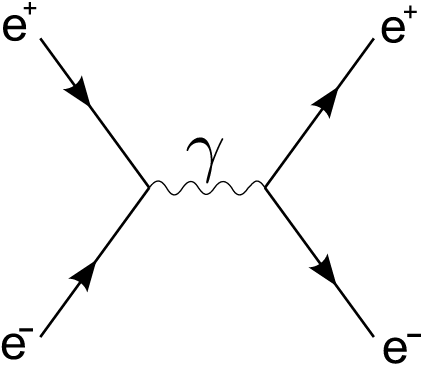
\includegraphics[width=0.35\textwidth]{fig/chapt2/electromagnetic.png}
%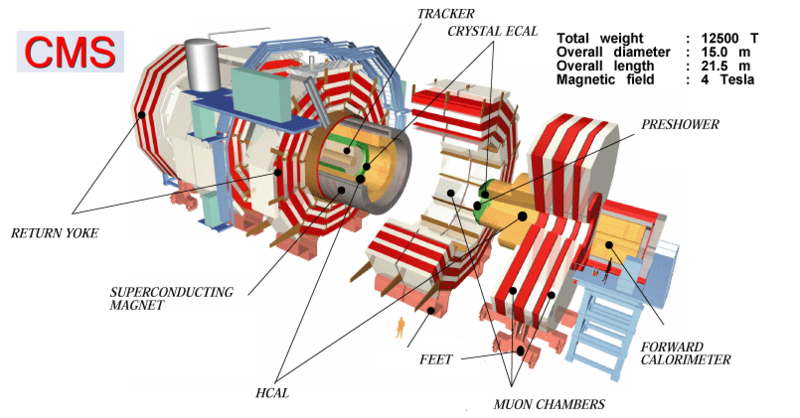
\includegraphics[scale=0.4, trim=20 50 60 30,clip]{fig/chapt3/CMS_exper.png}
\caption{\label{fig:electro_force} An overview of the Bhabha scattering in QED.}
\end{figure}
\item{\textbf{Weak Interaction}}:
All fundamental particles except gluon (g) and photon ($\gamma$) experience undergoes weak interaction by exchanging or producing W$^{\pm}$ or Z bosons. It is a short range (10$^{-17}$ to 10$^{-16}$m) interaction and responsible for many phenomena like radioactivity and quark spin flipping. Weak isospin (Y$_{3}$) conserves in weak interaction and plays a similar role in weak interaction as colour in strong interaction and charge in electromagnetism. In case of leptons, the theory is very clear, like the decay of muon mediated by W$^{-}$ boson ($\mu^{-} \rightarrow e^{-} + \nu_{\mu} + \bar{\nu_{e}}$) and electron-neutrino scattering via Z boson ($\nu_{\mu} + e^{-} \rightarrow \nu_{\mu} + e^{-}$). The lepton number conserve in both processes. A similar model applied to the three generation of quarks where a quark converts into same generation but in nature across generation conversion observed. The dilemma was solved by introducing the 3 $\times$ 3 $\textbf{CKM}$ (Cabibbo–Kobayashi–Maskawa) matrix \ref{eq:ckm1}, very near to unitary.
\begin{equation}\label{eq:ckm1}
\left({\begin{array}{ccc} \rm d' \\ \rm s' \\ \rm b' \end{array}}\right) = 
	  \left( \begin{array}{ccc}
      \rm  V_{ud} &\rm V_{us} &\rm V_{ub}\\
      \rm  V_{cd} &\rm V_{cs} &\rm V_{cb}\\
      \rm  V_{td} &\rm V_{ts} &\rm V_{tb}\end{array} \right)
\left({\begin{array}{ccc} \rm d \\ \rm s \\ \rm b \end{array}}\right)
\end{equation}  
The down type quarks ($\rm d', \rm s', \rm b'$) is a superposition of down type quarks following Equ.\ref{eq:ckm1} and couple to up type quarks via charged current weak interaction. The matrix elements gives the rate at which one quark convert to another e.g $\rm V_{ud}$ gives the transition rate of $d \rightarrow u$. All the nine CKM matrix values are given in \ref{eq:ckm2}.
\begin{equation}\label{eq:ckm2}    \small 
\rm V_{\rm CKM}	=  \left( \begin{array}{ccc}
      \rm  0.97434_{-0.00012}^{+0.00011} &\rm 0.22506\pm 0.0005&\rm 0.00357\pm 0.00015\\
      \rm  0.22492\pm 0.0005 &\rm 0.97351\pm 0.00013 &\rm 0.0411\pm 0.0013\\
      \rm  0.00875_{-0.00033}^{+0.00032} &\rm 0.0403\pm 0.0013 &\rm 0.99915\pm 0.00005\end{array} \right)
\end{equation}
The diagonal elements are $\approx$1, show the transition in the same generation is dominant \cite{ckm}.\item{\textbf{The Electroweak Symmetry:}}
The electromagnetic and weak forces were combined by Glashow, Weinberg and Salam in a unique gauge electroweak theory (GWS) based upon the $SU(2)_{L}\times U(1)_{Y}$ group \cite{gws}. The theory introduces three SU(2)$_{L}$ gauge bosons W$^{i}_{\mu}$, i = 1,2,3, with coupling strength g$_{w}$ and one U(1)$_{Y}$ gauge boson, B$_{\mu}$ with coupling constant g$'$/2. The GWS theory depends upon the chirality of particles that means it transforms left-handed particles as doublets with weak isospin (I) $\pm\frac{1}{2}$ and right-handed particles as singlet with I = 0. The hypercharge (Y) and the third component of weak isospin (I$^{3}$) are related to charge (Q in unit of e) as:
\begin{equation}\label{eq:}
Q = I^{3} + \frac{1}{2}Y
\end{equation}  
The wave function of the charged fields W$^{\pm}_{\mu}$, neutral field Z$_{\mu}$ and photon A$_{\mu}$ is represented by:
\begin{equation}\label{eq:electroweak}
\begin{split}
W^{\pm}_{\mu} = \frac{1}{\sqrt{2}}\left( W_{\mu}^{1} \mp W_{\mu}^{2}\right)\\
Z_{\mu} = \left( W_{\mu}^{3}\cos\theta_{w} - B_{\mu}\sin\theta_{w}\right)\\
A_{\mu} = \left( W_{\mu}^{3}\sin\theta_{w} + B_{\mu}\cos\theta_{w}\right)
\end{split}
\end{equation}   
where $\theta_{w}$ is the weak mixing angle given in term of electromagnetic coupling constant (g$_{e}$) as:
\begin{equation}
g_{w}\sin\theta_{w} = g'\cos\theta_{w} = g_{e} 
\end{equation} 
In GWS theory, breaking of the underlying $SU(2)_{L}\times U(1)_{Y}$ symmetry predicts the existence of two charged guage fields and two neutral guage fields shown in Equ.\ref{eq:electroweak}.  
\item{\label{item:higgs_mechanism}\textbf{The Higgs Mechanism:}} SM is based on gauge invariance which forbids to introduce explicit mass terms in the Lagrangian of a chiral theory, as it breaks the symmetry. This results to massless SM particles, a contradiction to the nature. A mechanism is needed to introduce mass term in the SM without spoiling guage symmetry known as Higgs Mechanism also called Brout-Englert-Higgs (BEH) mechanism \cite{eng_brout,p_w_higgs}. The GWS uses the BEH mechanism which introduces a new doublet of complex scalar field, known as Higgs field, preserves symmetry under the gauge transformations, and acquires a non-zero vacuum expectation value, spontaneous electroweak symmetry breaking. The Higgs field contains a total of four additional degrees of freedom where three of them become massive, given in \ref{eq:electroweak}, after breaking the symmetry and one remains massless, the photon $\gamma$. The Higgs doublet introduces in the SU(2)$_{L}$ with hypercharge (Y = $\frac{1}{2}$) is in the form of,
\begin{equation}
\phi = \Big(\begin{array}{c}
\phi^{+}\\
\phi^{0} \end{array}\Big)
= \frac{1}{\sqrt{2}}
\Big(\begin{array}{c}
\phi^{1} + i\phi^{2}\\
\phi^{3} + i\phi^{4}
\end{array}\Big)
\end{equation}
The SM electroweak Lagrangian density is given in term of
\begin{equation}\label{eq:beh_lagrange}
\mathcal{L}_{BEH} = (D^{\mu}\phi)^{\dagger}(D_{\mu}\phi) - V(\phi), \quad \textrm{with}\quad 
        V(\phi) = \mu^{2}\phi^{\dagger}\phi + \lambda(\phi^{\dagger}\phi)^{2}
\end{equation}
where first term of the lagrangian D$^{\mu}$ corresponds to the covariant derivative of the Higgs field under the SU(2) $\times$ U(1) group and the second term is the scalar potential known as "Mexican Hat" potential, shown graphically in Fig.\ref{fig:mexican_hat}. 
\begin{figure}[h]
\centering
\captionsetup{width=0.8\linewidth}
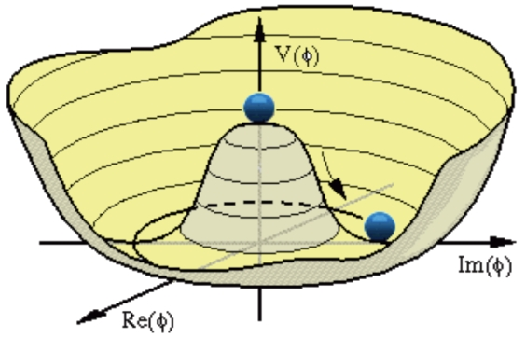
\includegraphics[width=0.4\textwidth]{fig/chapt2/mexican_hat.png}
%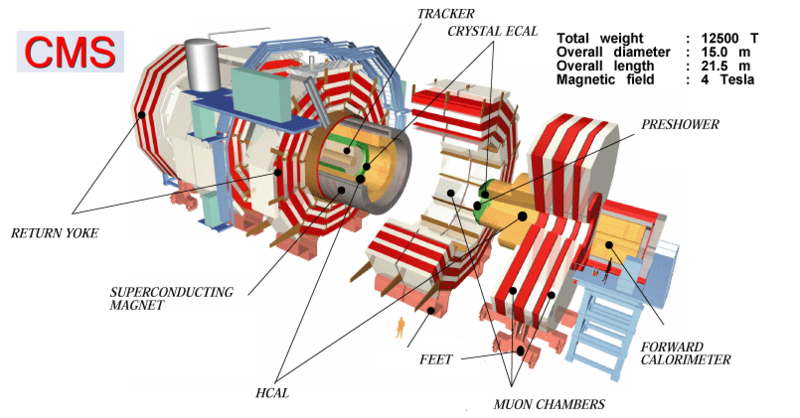
\includegraphics[scale=0.4, trim=20 50 60 30,clip]{fig/chapt3/CMS_exper.png}
\caption{\label{fig:mexican_hat}The scalar potential V($\phi$)with $\mu^{2}$ < 0 has a "Mexican hat shape, with the minimum in a rim around the origin. Moving from the origin down to the minimun, the symmetry breaks and the scalar field acquire a vacuum expectation value (vev) in the process}
\end{figure}
The higgs potential has chosen in the simplest form to achieve the necessary spontaneous symmetry breaking, while being renormalizable. The Higgs potential V($\phi$) depends on the values of $\lambda$ and $\mu^{2}$. For a stable vacuum, the parameter $\lambda$ has to be a positive value. If $\mu^{2}$ > 0, the scalar potential has a global minimum, $\langle 0\abs{\phi}0\rangle = 0$, where no spontaneous symmetry breaking occurs; while for $\mu^{2} < 0$ the symmetry breaks and the Higgs field acquires a non zero vacuum expectation value with conditions $\langle 0\abs{\phi}0\rangle = \frac{-\mu^{2}}{2\lambda} = \frac{\nu}{\sqrt{2}}$ where $\nu = \sqrt{-\frac{\mu^{2}}{\lambda}}$ is the vev. The scale of electroweak symmetry breaking is related to the W boson mass and to the Fermi constant G$_{F}$:
\begin{equation}
\nu = 2\frac{m_{w}}{g_{w}} = (\sqrt{2}G_{F})^{-\frac{1}{2}} \approx 240 GeV 
\end{equation}
The Higgs field can be re-defined in terms of a perturbation around its non-zero vev by inserting a new scalar field h(x):
\begin{equation}\label{eq:higgs_state}
\phi(x) = \frac{1}{2}\left(\begin{array}{c}
0\\
\nu + h(x)
\end{array}\right)
\end{equation}
The new scalar field corresponds to the Higgs particle with mass $m_{h} = \nu\sqrt{2\lambda}$ and no charge. Rearranging Equ.\ref{eq:beh_lagrange} by inserting $\phi$ from \ref{eq:higgs_state} and defining the bosonic states shown in \ref{eq:electroweak} we can see that the three bosons (W$^{\pm}$, Z$^{0}$) acquire masses while photon $\gamma$ remains massless.
\begin{equation}
m_{W}^{2} = \frac{\nu^{2}g^{2}}{4} ; m_{Z}^{2} = \frac{\nu^{2}(g^{2} + g'^{2})}{4} ; m_{\gamma} = 0 
\end{equation}
The concept of the gauge boson mass terms can be further extended to the mass terms of the fermions in a different way that would also break the local gauge invariance of the theory. This can be done by introducing the Yukawa coupling $\lambda_{f}$ between the fermions fields and the Higgs boson with the coupling constant proportional to the respective fermion mass. We get,
\begin{equation}
m_{f} = \frac{\lambda_{f}}{\sqrt{2}}\nu
\end{equation}
In SM, neutrinos are considered massless.
The Higgs mechanism successfully serves in the GWS model to give masses to weak bosons and predict a new scalar particle, the Higgs boson. In 2012, both CMS and ATLAS discovered the Higgs boson that confirmed the symmetry breaking in nature.
\end{itemize}

\subsection{The Top Quark}
Top quark belongs to the third generation of quarks, the heaviest known elementary particle in the SM, and with its unique properties has long been considered of potentially carrying key information that may lead to answer some of the basic open questions in particle physics. The CDF and D0 collaborations at the Tevatron in 1995 bring the long quest of the sixth and last quark of the SM to an end by the discovery of top quark \cite{top_quark}. The mass of the top quark measured to be 173.5 and has very short life time $\approx$ 10$^{-23}$s, less than the time of hadronization that enables the top quark to decay before forming bound state. The LHC started data taking in 2010 at $\sqrt{s}$ = 7 TeV and after the three years of data taking by CMS and ATLAS, about a million of top quark events we recorded which named the LHC as “top factory”. All the current results of the top quark production, decay and coupling are consistent with the Standard Model prediction and no clue of physics beyond Standard Model have been observed in its properties. However different studies are underway to search for new physics especially in the $t\bar{t}$ resonance and interference production. The interference pattern comes into play when the SM $t\bar{t}$ background interfere with the signal (decay of the scalar or pseudo-scalar into $t\bar{t}$). The focus of this thesis is the search for heavy scalar and pseudo-scalar decaying into $t\bar{t}$ where $t\bar{t}$ further decays leptonically. Both resonance and interference are studied in detail. 
\begin{figure}[h]
\centering
%\captionsetup{width=0.8\linewidth}
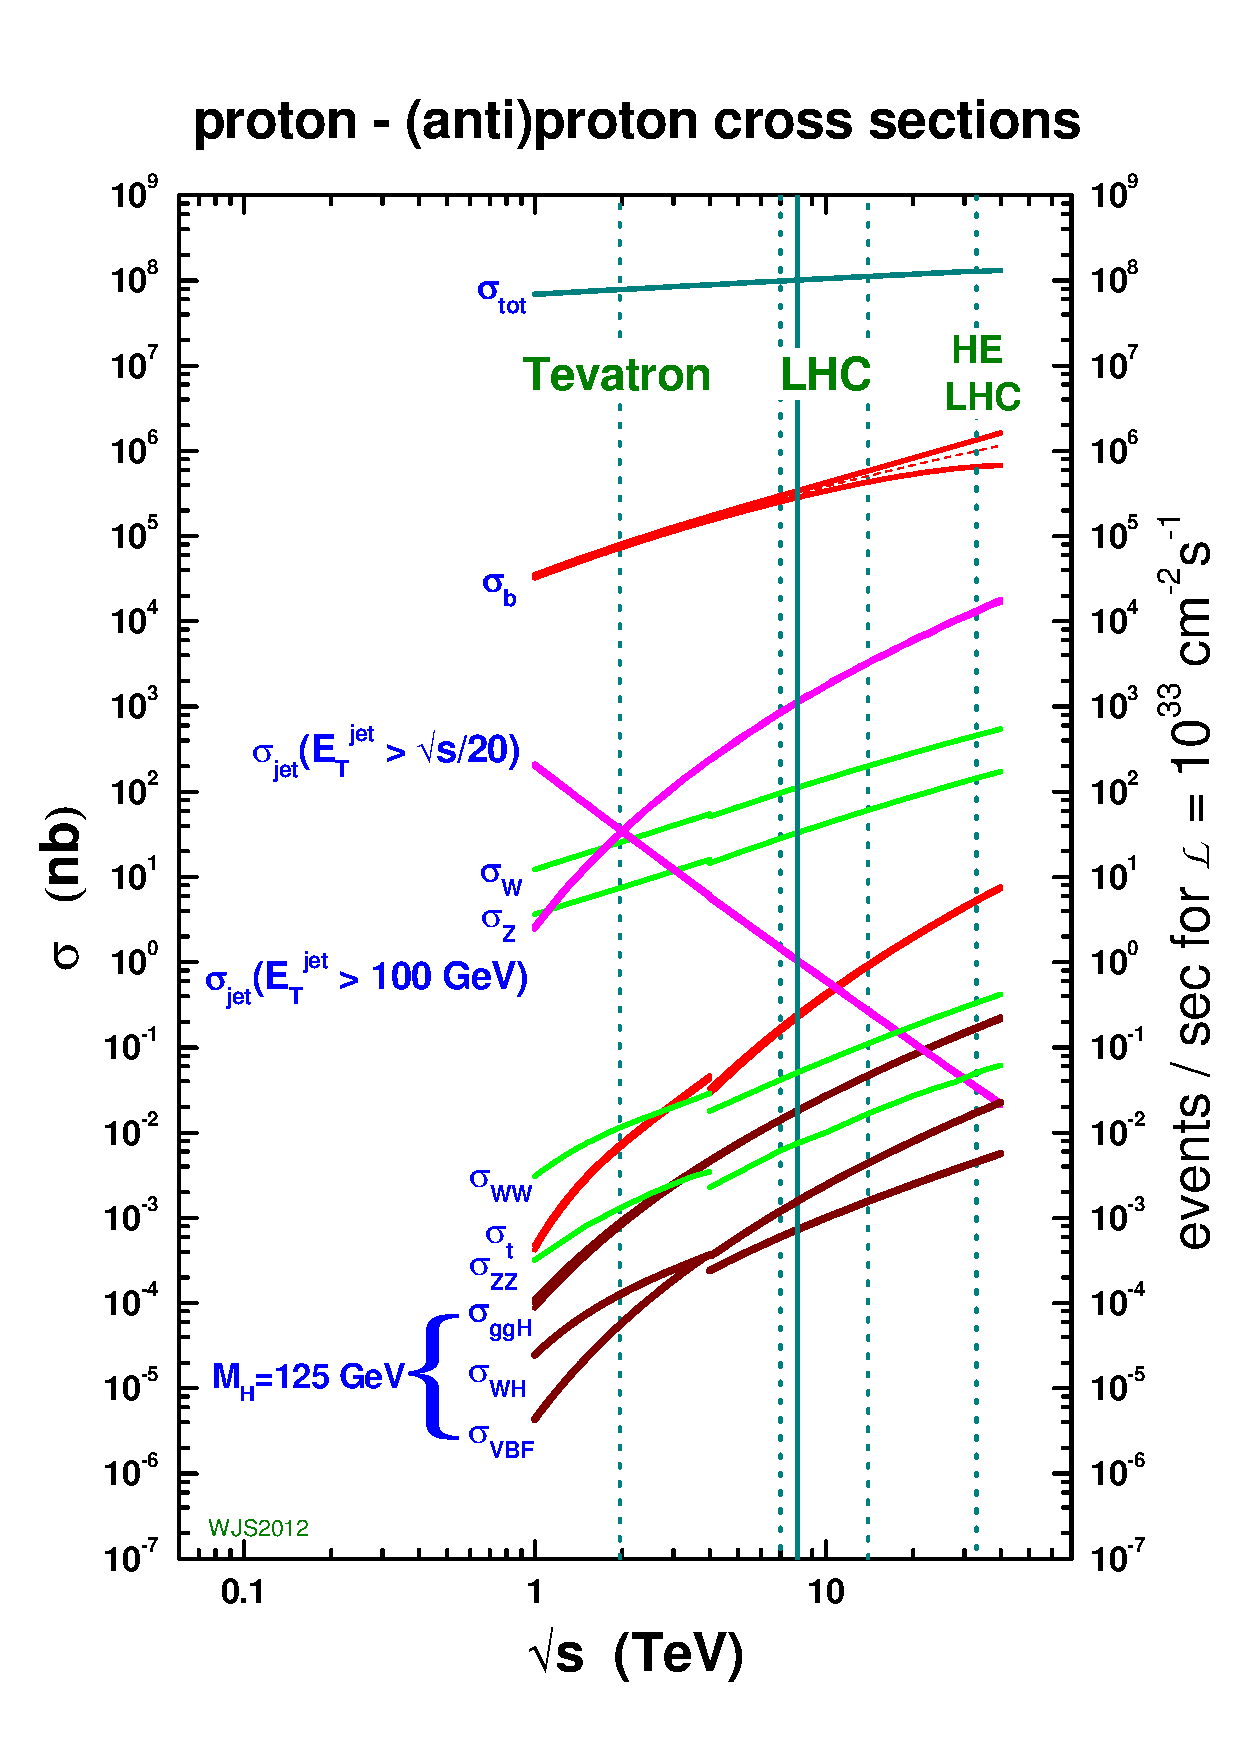
\includegraphics[width=0.6\textwidth]{fig/chapt2/crosssections2012HE_v4.pdf}
%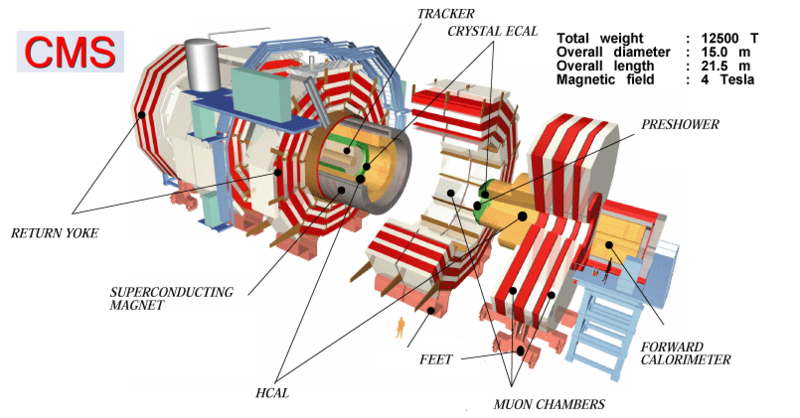
\includegraphics[scale=0.4, trim=20 50 60 30,clip]{fig/chapt3/CMS_exper.png}
\caption{\label{fig:lhclumi_plot}The Standard Model cross sections as a function of energy \cite{lhclumi_plot}.}
\end{figure}
\subsubsection*{Top quark production}
At hadron colliders, two mechanisms are responsible for the top quark production, $t\bar{t}$ pairs via strong interaction and single top production via electroweak process, where $t\bar{t}$  is the most abundant production at high energy regime. The production of $t\bar{t}$ is contributed by the two LO processes at tree level shown in Fig.\ref{fig:ttbar_prod}: quark–antiquark ($q\bar{q}$) annihilation and gluon–gluon (gg) fusion in the s-, t-, and u-channel. In $p\bar{p}$ collider such as Tevatron, the dominant production mode for $t\bar{t}$ is the $q\bar{q}$ annihilation while for $pp$ collider like LHC, $gg$ fusion more likely takes place. The hadronic production cross section of the $t\bar{t}$ pair is successfully explained by the QCD and obtained from the proton-proton interaction using the factorization theorem \cite{ttbar_production} read as:
\begin{equation}
d\sigma_{pp\rightarrow t\bar{t}}(s,m_{t}) = \sum\limits_{i,j=q,\bar{q},g}\int dx_{i}dx_{j}f_{i}(x_{i},\mu^{2}_{f})f_{j}(x_{j},\mu^{2}_{f}).\hat{\sigma}_{ij\rightarrow t\bar{t}}(\hat{s}, m_{t}, \mu_{f},\mu_{r}, \alpha_{s}))
\end{equation}
The cross sections are integrated over all partons participating in the scattering process with momentum fractions x$_i$ and x$_j$ with respect to the proton momenta and summed over all parton type i and j. The PDFs $f_{i}(x_{i}, \mu^{2}_{f})$ are partonic distribution functions, describe the probability to find a parton i inside a hadron in momentum range x to x+dx. The PDFs absorbs all types of long-distance effects of partons inside the hadrons whereas the hard scattering partonic cross section $\hat{\sigma}$ represents the actual hard process at small distances which can be computed in perturbative QCD. The long and short distance processes can be separated by introducing a new energy scale called “factorization scale ($\mu_{f}$)” on which both PDFs and $\hat{\sigma}$ depend. The hard scattering partonic cross section $\hat{\sigma}$ further depends on the partonic center-of-mass energy $\hat{s} = x_{i}x_{j}s$ (s is the pp CoM energy squared), the renormalization scale $\mu_{r}$, to treat ultraviolet divergence, and the strong coupling constant $\alpha_{s}$. Both energy scales, $\mu_{f}$ and $\mu_{r}$, are set to the physical energy scale of the process, like for $t\bar{t}$ pair production cross section, they are set to the top quark mass; $\mu_{f} = \mu_{r} = m_{t}$. The recent measurement of $\sigma(t\bar{t})$ at CMS resulted 889 $\pm$ 2 (stat)$^{+26}_{-28}$ (syst) $\pm$ 20 (lumi) pb,  in agreement with the standard model prediction\cite{top:16_006}.\\
\begin{figure}[h]
\centering
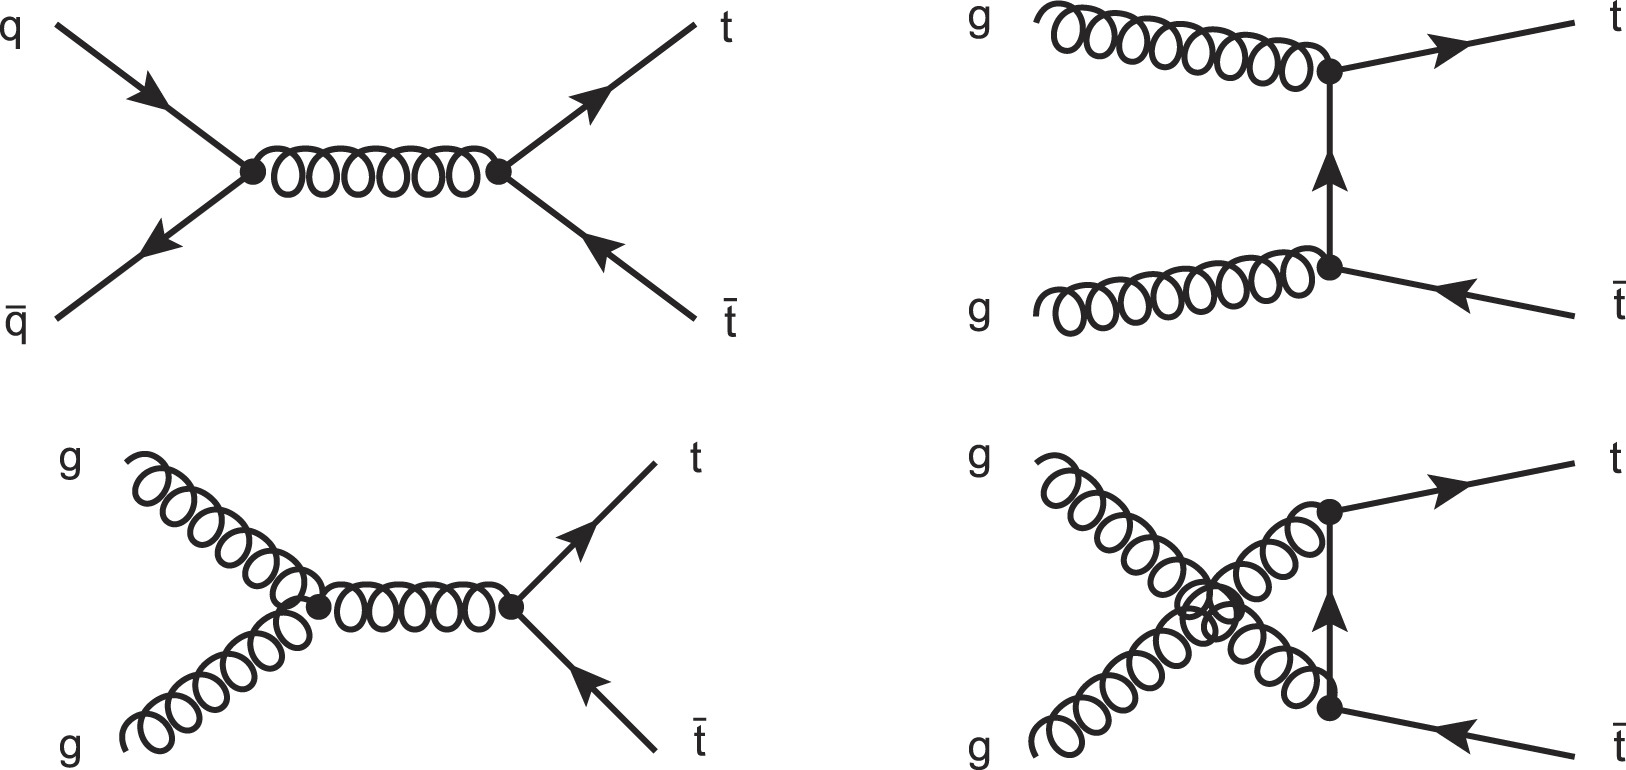
\includegraphics[width=0.7\textwidth]{fig/chapt2/ttbar_productions.jpg}
\caption{\label{fig:ttbar_prod}$t\bar{t}$ pair production in QCD at LO: top left is $q\bar{q}$ annihilation, bottom left is gg fusion in the s-channel, top right is gg fusion in the t-channel and bottom right shows gg fusion in the u-channel.}
\end{figure}
Single-top can be produced at hadron colliders via three different electroweak processes, t-channel (the dominant channel with 70\% of the total cross section), the associated production of a top ($\bar{t}$) quark and a W boson (tW-channel with 25\% cross section) and the s-channel (5\% of the total cross section). The electroweak production vertex includes the CKM matrix element V$_{tb}$ that makes the single top processes more interesting for SM and BSM physics.
\subsubsection*{Top quark decay}
The top quark almost exclusively decays into a W-boson and a b-quark via the electroweak interaction due to the CKM matrix element V$_{tb} \approx$ 1. Compare to other quarks of the SM, top quark has very short life time ($\tau_{t} \approx 5 \times 10^{-25}$s) and decays before hadronization ($\tau_{had} \approx 10^{-24}s$). This makes the top quark more interesting to be studied in bare state and its kinematic and dynamic information, like spin correlation, transfers to its decay products without diluted by hadronization. The decay of $t\bar{t}$ system can be classified on the basis of W boson decay products where W boson can decay into a pair of light quarks, with BR($W \rightarrow q\bar{q}') \simeq 67\%$, or charged leptons with corresponding neutrino of the same generations with BR($W \rightarrow l\nu_{l}) \simeq 33\%$. At first order, the possible decay modes of a $t\bar{t}$ event can be grouped into three main categories given in table\ref{table:ttbar_decay}
\begin{table}[h]%\footnotesize
\centering
     %\begin{tabular}{|p{1.4cm}|p{1.0cm}|p{1.0cm}|}
    \tabulinesep=1.0mm
     \begin{tabu}{|l|c|c|}
        \hline
        Channel & Decay mode & BR\\
\hline 
Hadronic & $t\bar{t}\rightarrow b\bar{b}W^{+}W^{-}\rightarrow b\bar{b}q\bar{q}'q''\bar{q}'''$ & 46\%\\ 
\hline
Semileptonic & $t\bar{t}\rightarrow b\bar{b}W^{+}W^{-}\rightarrow b\bar{b}q\bar{q}'l\nu_{l}$ & 45\%\\ 
\hline
Dileptonic & $t\bar{t}\rightarrow b\bar{b}W^{+}W^{-}\rightarrow b\bar{b}ll'\nu_{l}\nu_{l'}$ & 9\%\\
\hline
\end{tabu}
     \caption{Three categories of $t\bar{t}$ sytem decay with branching ratios\cite{ttbar_decay_ratio}.\label{table:ttbar_decay}}
%\end{center}
\end{table}  

\begin{figure}[htp]
\centering
\begin{tabular}{cc}
\hspace{-0.3cm}
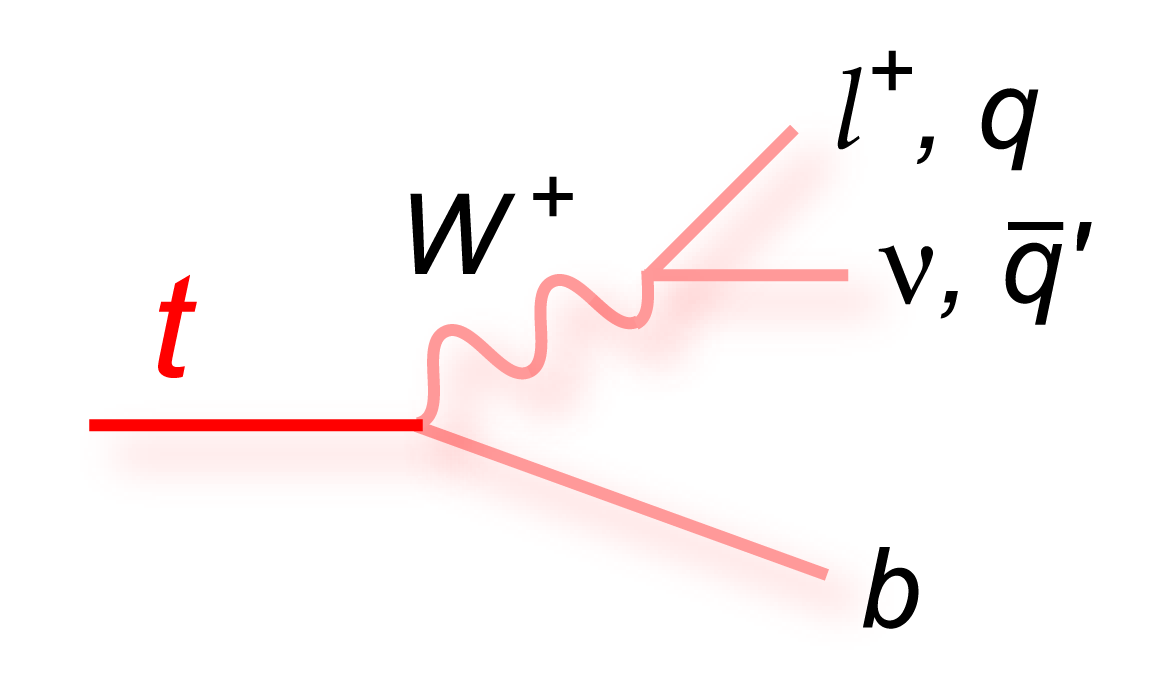
\includegraphics[scale=0.19]{fig/chapt2/single_top_decay.png}
& \hspace{-0.5cm} 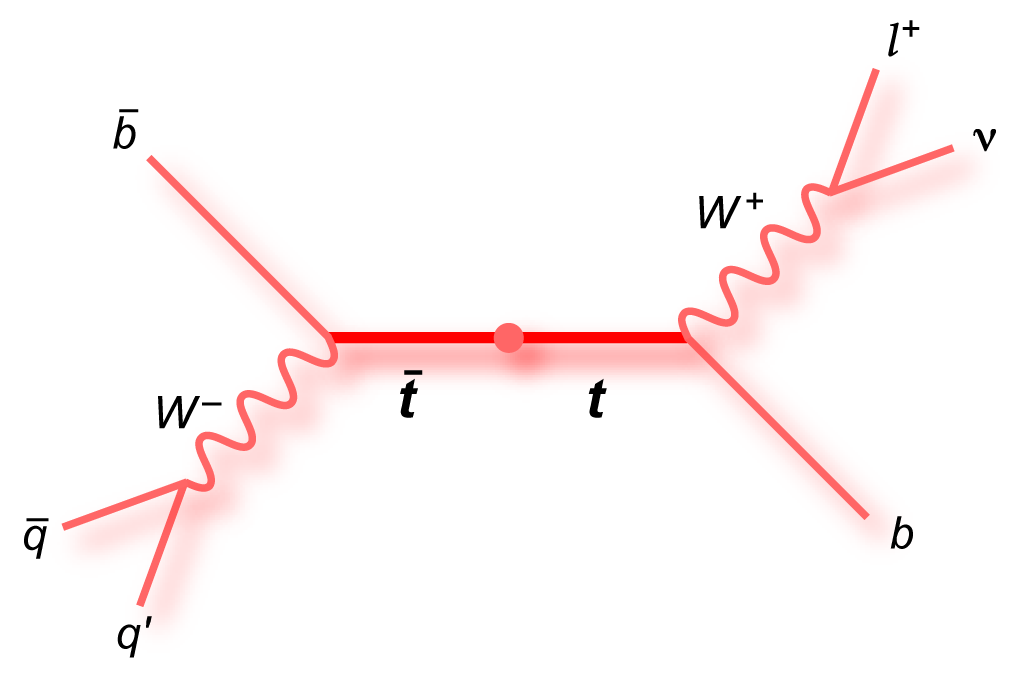
\includegraphics[scale=0.19]{fig/chapt2/ttbar_decay.png}\\
   ($\mathbf{a}$)\qquad\qquad\qquad&($\mathbf{b}$)\qquad\\
\end{tabular}
\caption{Feynman diagram for sigle top quark decay (a) and the semileptonic decay of $t\bar{t} $ (b).}\label{fig:top_decay}
\end{figure}
\begin{itemize}
\item {\textbf{Hadronic Channel:}}
Both W bosons coming from $t\bar{t}$ event decay into light quark-antiquark pairs (quark and antiquark further hadronized in the form of jets) with high branching fraction, resulted to a large sample of selected events. In this channel at least six jets are needed, two of them are stemming from bjets and remaining from light jets. In hadron colliders like LHC, this channel  suffers from an overwhelming QCD multijet background, whose cross section is orders of magnitude higher than the one for $t\bar{t}$ production. The QCD multijet background is difficult to model from simulation which requires data driven technique to take it from data.
\item{\textbf{Dileptonic Channel:}}
In dileptonic channel, both of W bosons decay leptonically, resulting two bjets, two charged leptons and two corresponding neutrinos in $t\bar{t}$ event. It has the lowest branching ratio but a very clean signature at the experimental level due to the presence of two oppositely charged leptons, which can be easily distinguished from QCD multijet events. The disadvantage of dileptonic event is the presence of two neutrinos, considered as the missing transverse energy in the event, where $t\bar{t}$ can’t be reconstructed perfectly. 
\item{\textbf{Semileptonic Channel:}}
Finally, the lepton+jets channel whose decay chain is shown in Fig.\ref{fig:top_decay}b, is a good compromise between a reasonable
BR and relatively clean experimental signature with reconstructable tt-event topology (especially when lepton = $\mu$, e). The semileptonic channel is restricted to $\mu$ + jets and e + jets as the $\tau$ lepton further decay into charged lepton and neutrino or jets which makes the channel more complicated. Therefore a dedicated study is needed to take into account the $\tau$ + jets channel.
 
With clean signature and adequate BR ($\sim$30\%), the lepton+jets channel has chosen for this thesis. In the resolved case, where final products of each top quark ($P_{T} \le 400GeV$) are reconstructed as separate objects, the $t\bar{t}$ final objects consists of four jets, one charged lepton (muon or electron) and neutrino. Two of the jets are tagged as bjets, arise directly from the decay of top quark while two of light jets coming from one of the W-boson. The second W-boson decays into a charged lepton and corresponding neutrino. As neutrino escapes without detection, it is treaded as missing transverse energy ($E^{miss}_{T}$) in the event. The longitudinal component of $E^{miss}_{T}$ is unmeasured which can be reconstructed using analytical solution explained in detail in Sec.\ref{https://arxiv.org/pdf/1305.1878.pdf}. The $t\bar{t}$ system is reconstructed using Rochester Algorithm explained in Sec.\ref{https://cds.cern.ch/record/2141097/files/TOP-16-008-pas.pdf}.      
\end{itemize}
\subsection{The SM Higgs Boson}
In early 60's, the existence of the Higgs boson was theoretically predicted by Robert Brout, Fran\c cois Englert and Peter Higgs using the well known BEH mechanism \ref{item:higgs_mechanism}. The main goal in the field of particle physics during the last few decades was the Higgs boson discovery, where a number of searches have been conducted at the Large Electron-Positron Collider (LEP) at CERN and at Fermilab with the experiments CDF and D0 at $\sqrt{s} = 1.96$ TeV using an integrated luminosity of 10.0 fb$^{-1}$. The later narrowed down the mass range by excluding two regions: 100 < m$_{H}$ < 130 GeV/c$^{2}$ and 147 < m$_{H}$ < 180 GeV/c$^{2}$, at the 95\% C.L. Furthermore, they observed a significant access of data events with respect to the background estimation in the
mass range, 115 < m$_{H}$ < 140 GeV/c$^{2}$ \cite{sm_higgs_fermilab}. The official announcement of the higgs boson discovery with 5$\sigma$ significance made by the CERN experiments, CMS and ATLAS, in July 2012 by combining data of 7 and 8 TeV energy with integrated luminosity of 10.4 fb$^{-1}$ by CMS and 10.6 fb$^{-1}$ by ATLAS \cite{cms_sm_higgs,atlas_sm_higgs}. The search performed in five higgs decay modes: $\gamma\gamma$, ZZ, W$^{+}$W$^{-}$, $\tau^{+}\tau^{-}$ and $b\bar{b}$ where excess is most significant in the two decay modes with the best mass resolution, $\gamma\gamma$ and ZZ. By performing a fit to the signals, the mass of the higgs boson is 125.3$\pm$0.4(stat.)$\pm$0.5(syst.) GeV. At 13 TeV, the study has been repeated and the mass of the higgs boson measured to be 124.50$^{+0.48}_{-0.46}$ GeV with a constrained on width $\Gamma_{H}$ < 41 MeV \cite{sm_higgs_13tev}. The measured cross section agrees well with the expectation from the standard model. The signal strength $\mu$, defined as the production cross section of the Higgs boson times its branching fraction to four leptons relative to the standard model expectation, is measured to be; $\mu$ = 0.99$^{+0.33}_{-0.26}$ at m$_{H}$ = 125.09 GeV. The higgs boson properties like spin, parity, the ratios of production rates for different production modes, the ratios of couplings to fermions and vector bosons etcetera are well agree with the standard model prediction. The higgs mass measured at 13 TeV using 12.9 fb$^{-1}$ data in two channels $H\rightarrow\gamma\gamma$ (a) and $H\rightarrow ZZ\rightarrow 4l$ (b) is shown in figure \ref{fig:sm_higgs} where excess in data is clear around 125 GeV is visible. 
   
\begin{figure}[htp]
\centering
\begin{tabular}{cc}
\hspace{-0.3cm}
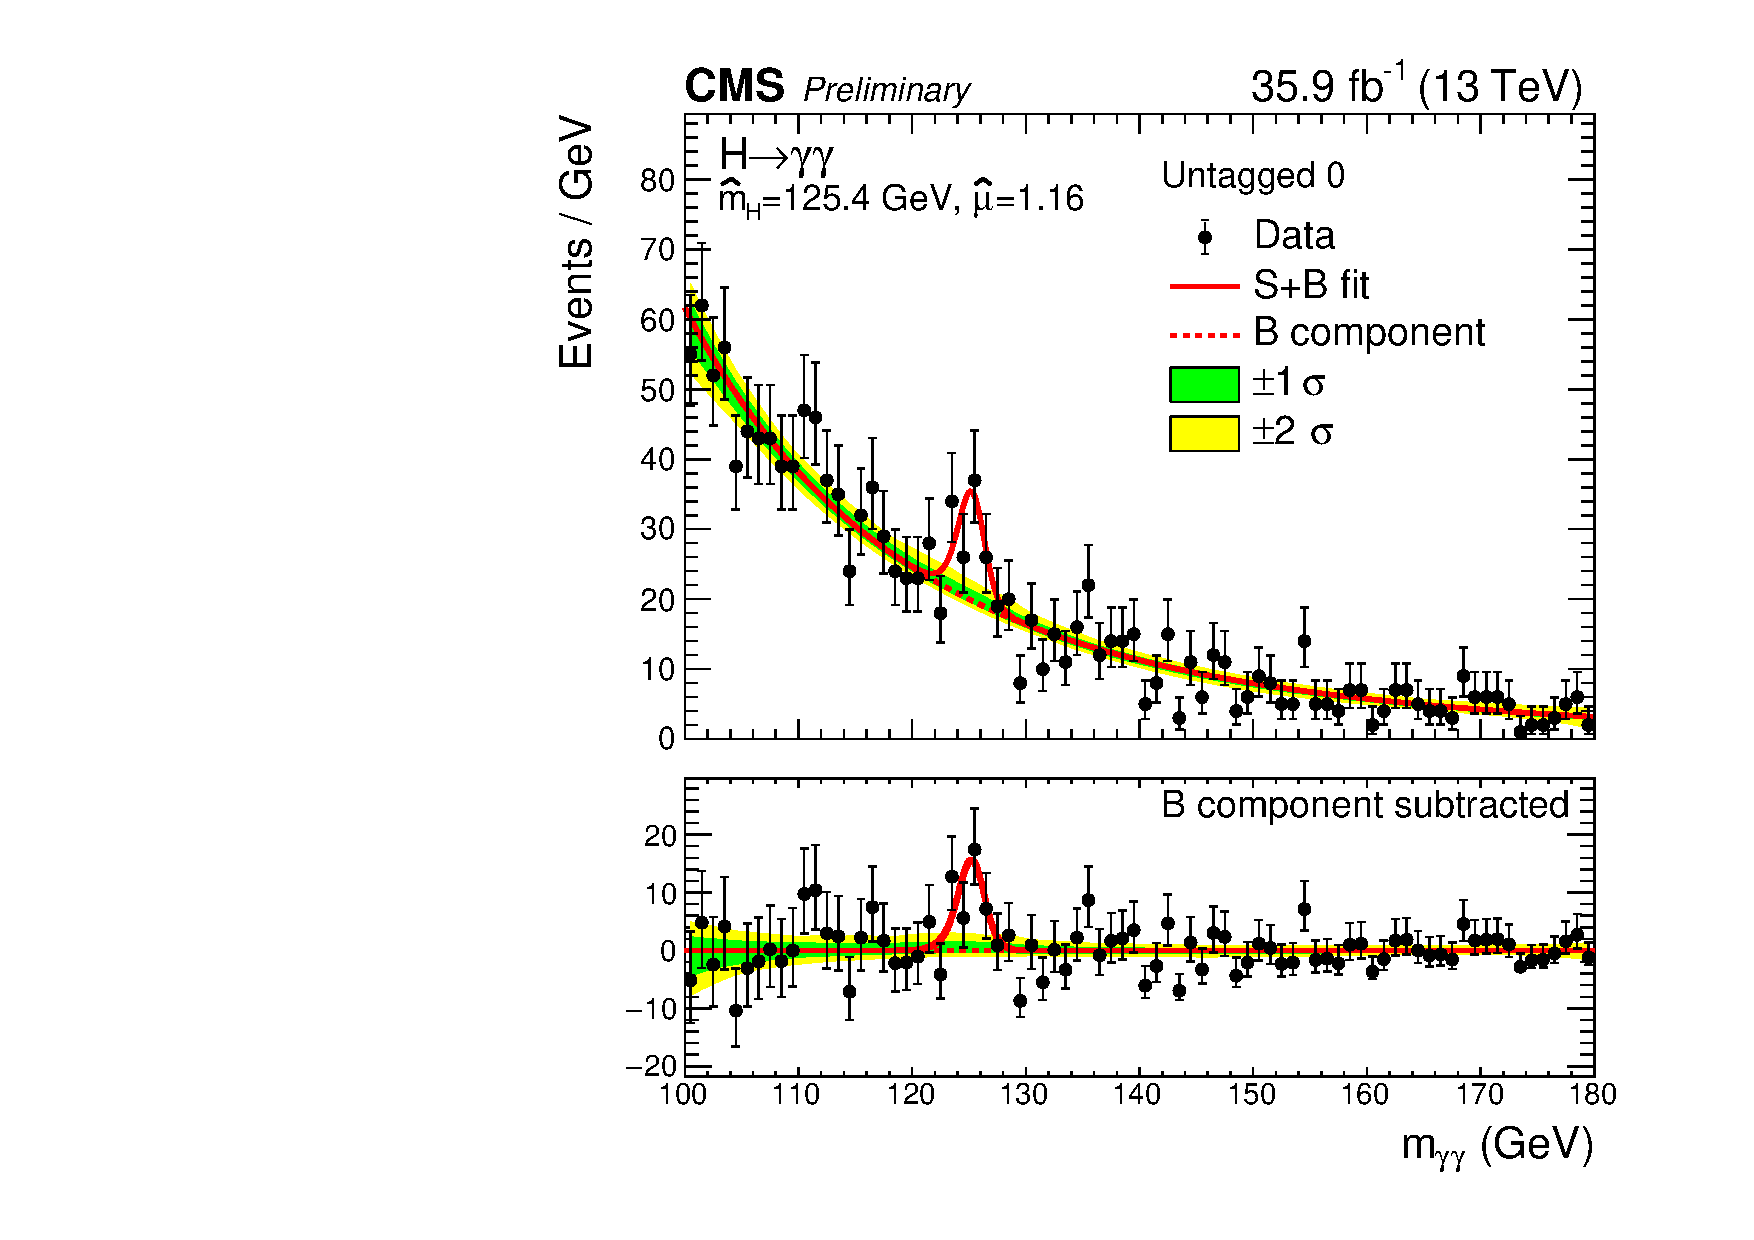
\includegraphics[scale=0.35]{fig/chapt2/CMS-PAS-Htogamma.pdf}
& \hspace{-0.5cm} 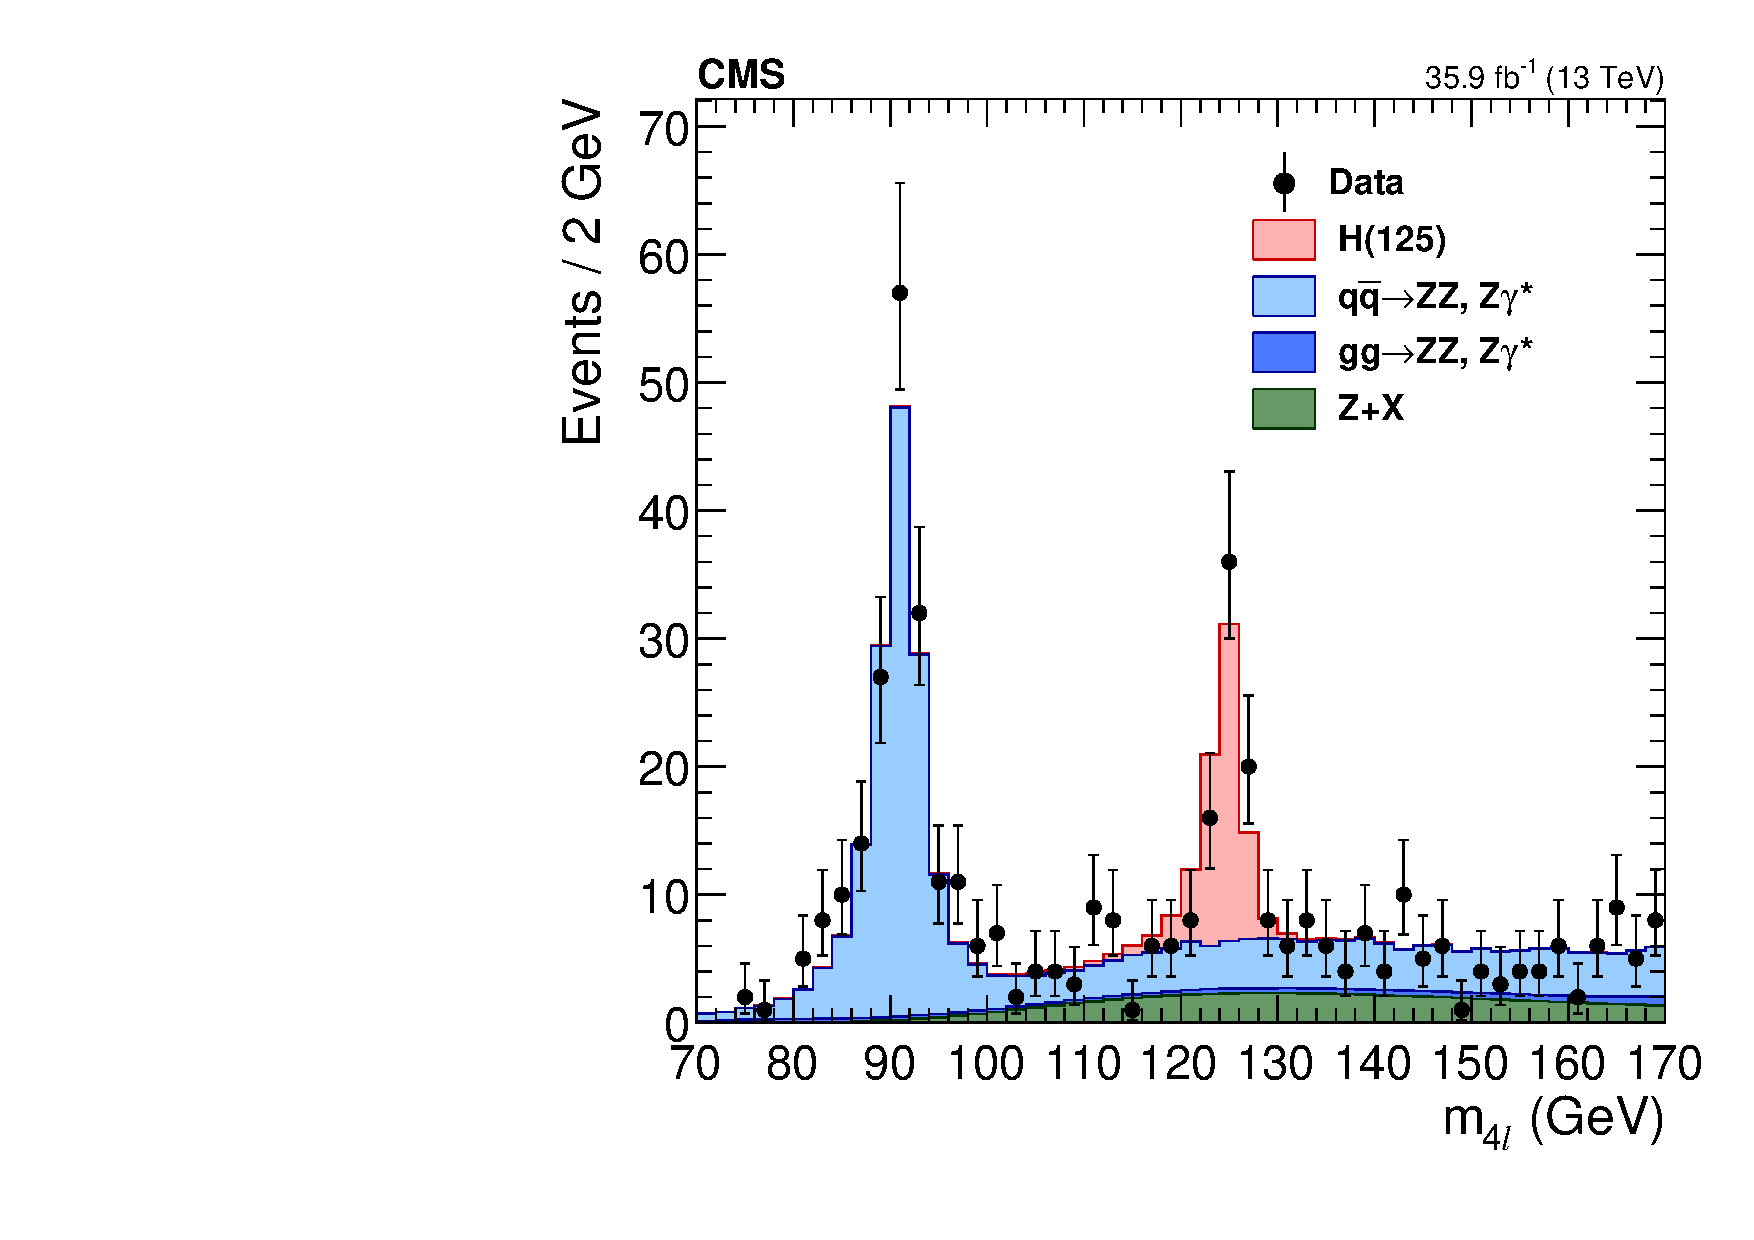
\includegraphics[scale=0.35]{fig/chapt2/CMS-PAS-Hto4l.pdf}\\
   ($\mathbf{a}$)\qquad&($\mathbf{b}$)\qquad\\
\end{tabular}
\caption{\label{fig:sm_higgs}The SM Higgs mass spectra obtained in the 2016 CMS search using the two most sensitive decay channels, di-photon (left) and four-lepton (right). Both channels show larger than 5 standard deviations significance of the observed signals around 125 GeV and the data correspond to an integrated luminosity of 13 fb$^{-1}$, collected with the CMS detector at a centre-of-mass energy of 13 TeV \cite{pub:sm_higgs4l,pub:sm_higgs2gamma}.}
\end{figure} 

\begin{itemize}
\item{\textbf{Production and decay of the SM Higgs boson:}} The SM higgs boson couples to every massive particle hence production in hadron collider is possible in many ways, following four of them are the most common.
\begin{enumerate}
\item{\textbf{Gluon-gluon fusion (ggF):}} In this mode of production, two gluons interact to produce a Higgs boson mediated by heavy quarks (mainly top quark) loop as higgs boson doesn't directly couple to massless gluon. This channel of production has higher cross section through out the higgs boson mass range.
\item{\textbf{Vector boson fusion (VBF):}} In VBF mode, two quarks from colliding protons radiate massive vector bosons (W or Z) and its fusion results into the Higgs boson production. It is the second highest cross section process with 10 times less than the ggH but has a clear signature because of the pure electroweak process. 
\item{\textbf{Associated production with W$^{\pm}$ or Z$^{0}$ (VH):}} This process also known as Higgs-Strahlung, the third highest cross section, in which a massive vector boson produced by the interacting of a valence quark with an antiquark from the sea and the massive vector boson further radiates a Higgs boson. This mode is helpful to test the higgs coupling with the massive vector boson.
\item{\textbf{Associated production with $t\bar{t}$ ($t\bar{t}$H):}} In this mode of production, the higgs is associated with heavy quarks pair like top quark pair which can be initiated either by gluon-gluon fusion or $q\bar{q}$ annihilation. This channel has smaller cross section but more interesting because of the direct coupling with the top quark.
\end{enumerate} 
Higgs boson decays through many channels either direct coupling to the final state massive particles or indirectly via boson or fermion loop in massless final state particles (photon, gluon). The decay channel $H\rightarrow b\bar{b}$ has the largest branching ratio (BR) but diluted by the irreducible QCD background which mimics the signal. The same is true for $H\rightarrow \tau\bar{\tau}$ channel where $\tau$ decays hadronically. Despite the low BRs, the two channels $H\rightarrow ZZ^{\star}\rightarrow 4l$ and $H\rightarrow \gamma\gamma$ show a very clear signature to the higgs and ultimately the higgs discovery became possible using these two channels. Figure \ref{fig:sm_higgsxsec_BR} (a) shows the higgs cross section as a function of centre of mass energy for m$_{H}$ = 125 GeV with a band of theoretical uncertainty and (b) shows the BRs as a function of higgs mass with a band of total uncertainty(\%).     
\end{itemize} 
\begin{figure}[htp]
\centering
\begin{tabular}{cc}
\hspace{-0.3cm}
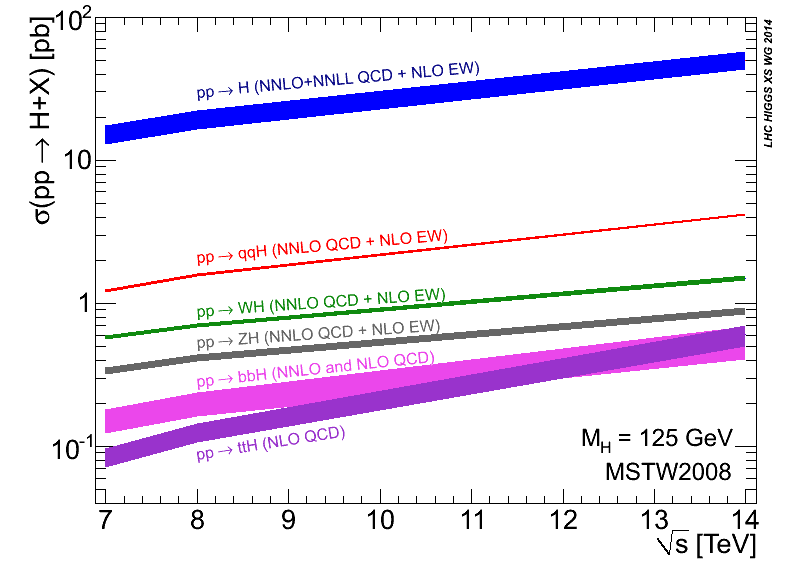
\includegraphics[scale=0.278]{fig/chapt2/7_14_xsec.png}
& \hspace{-0.5cm} 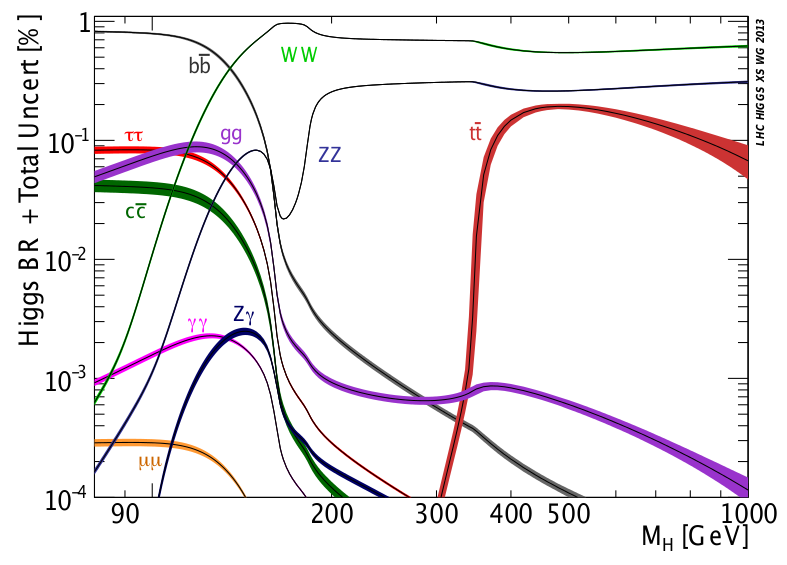
\includegraphics[scale=0.38]{fig/chapt2/Higgs_BR_RECT.png}\\
   ($\mathbf{a}$)\qquad&($\mathbf{b}$)\qquad\\
\end{tabular}
\caption{\label{fig:sm_higgsxsec_BR} Higgs boson (a): production cross section for main modes as a function of centre of mass energy exploiting m$_{H}$ = 125 GeV for $pp$ collider. (b): Branching ratio (BR) with full uncertainty in almost all channels as a function of higgs mass \cite{pub:sm_higgsxsec}.}
\end{figure} 
\section{Beyond the Standard Model}\label{sec:bsm}
Although the SM has been tested with great success in predicting and explaining many physics processes, especially in its gauge and flavour sector, but it is still not the ultimate theory as there exist a few experimental evidences and theoretical issues that are not explained by the SM. The most prominent among them are, the gravity, matter anti-matter asymmetry, the existence of dark matter and dark energy and the non-vanishing neutrino mass. There are some fundamental characteristics of the SM which we can't explain. The most important among them are: Why mass of the SM higgs boson is 125 GeV where the Plank scale is at $\mathcal{O}(10^{19})$ GeV?. This phenomenon is commonly known as hierarchy problem and a basic motivation for this search, explained in more detail in section \ref{subsec:hierarchy}. Why we have three families of fermion and they have a wide mass range?.
\subsection{The Hierarchy problem}\label{subsec:hierarchy}
Physics beyond the Standard Model can be probed by many reasons, but the core issue that is front and center for us today, relevant to Higgs boson physics and electroweak explorations at the Large Hadron Collider, is the Hierarchy Problem. The hierarchy problem involves the large difference between the Planck mass $M_{pl} \approx 10^{19}$ GeV, an energy scale associated with gravity, and the electroweak symmetry breaking scale ($10^{2}$) of the Standard Model. Higgs boson is the only fundamental scalar in the SM which can be subjected to higher order loops corrections from spin 0, 1/2 and 1 particles with a quadratic dependence on the cutoff scale (Plank scale). These corrections may take the higgs mass to the highest scale but in contrast we see the higgs mass $\sim$ 125 GeV. In case of fermions and guage bosons, their masses are protected by chiral and local guage symmetry respectively but for scalar higgs, there is no symmetry banning its mass term $m^{2}H^{\dagger}H$. Figure \ref{fig:higgs_massloop} upper row shows the quantum loop corrections to the higgs mass, left is the higgs self interaction, middle is the gauge boson loop and the right diagram shows the fermionic loop. In mathematical language, consider massive $N_{f}$ fermions with Youkawa coupling $\lambda = \sqrt{2}m_{f}/\nu$ and neglecting the external Higgs momentum squared, we obtain
\begin{equation}\label{equ:hierarchy}
\Delta M_{H}^{2} = N_{f}\frac{\lambda_{f}}{8\pi^{2}}\Big[\Lambda^{2} + 6m_{f}^{2}log\frac{\Lambda}{m_{f}} - 2m_{f}^{2} \Big] + \mathcal{O}(\frac{1}{\Lambda^{2}})
\end{equation}
where $\Delta M_{H}^{2}\propto \Lambda^{2}$. If we consider the cut off scale to be the Plank scale $M_{pl} \approx 10^{19}$ GeV, the Higgs boson mass becomes very huge which is against the experimental results. A counterterm $\mathcal{O}(10^{-30})$ needs to be added to the mass squared so that the value matches with the experimental result but this seems unnatural. This is commonly known as fine-tuning or naturalness \cite{hierarchy}. Several theories are proposed to cancel out infinities and leave the mass around the higgs mass (125 GeV). Supersymmetry (SUSY) is one of the leading possibility to solve the naturalness and hierarchy problem by introducing "superpartner" to the SM higgs particles. Such superpartners introducing additional feynman diagrams to cancel out the infinities as in figure \ref{fig:higgs_massloop} lower row for higgs, W boson and top quark.     
\begin{figure}[htp]
\centering
\hspace{-0.3cm}
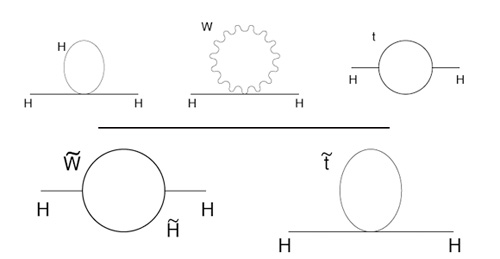
\includegraphics[scale=0.65]{fig/chapt2/higgs_mass_loop.jpg}
\caption{\label{fig:higgs_massloop}The three Feynman diagrams in top row from left to right represent higgs self coupling, W/Z boson and fermion (top quark) coupling respectively, a quantum effects on the Higgs mass. These effects boost the higgs mass to an infinite value which needs to be finite by using some unknown contributions. SUSY suggests supersymmetric partners of the Standard Model particles, one must include additional diagrams, where superpartners cancel out the loops effects in the higgs mass calculation as shown in the lower row. Source of the feynman diagrams is \cite{pub:higgsmassloop}.}
\end{figure}

\subsection{SuperSymmetry}
Supersymmetry (SUSY) is a space-time symmetry relating two different classes of particles, integer spin-0 and spin-1 (bosons) and spin-1/2 (fermions) \cite{phd_thesis:susy}. The SUSY generators $\mathcal{Q}$ transform a fermionic state into a bosonic state and vice–versa
\begin{equation}\label{equ:susy_gen}
\mathcal{Q}|Fermion\rangle = |Boson\rangle, \mathcal{Q}|Boson\rangle = |Fermion\rangle
\end{equation}
When the symmetry is exact, bosons and fermions have the same masses and quantum numbers, except for the spin. But the question arises, why we didn't find the superpartners of the SM particles? For examples electron discovered more than a century ago, if it has a superpartner with same mass and charge with opposite spin, it should to be discovered with simple experiments. Similarly no squark (where "s" stands for superpartner) has been observed in hadron-hadron colliders so for. This suggests that SUSY is not exact symmetry and must be broken in such a way that the superpartners acquire higher masses (higher than the top quark mass) but not too much high to reintroduce the hierarchy problem. This is commonly known as "soft" breaking of the SUSY. Up to now nobody has found a complete satisfactory dynamical way to break SUSY but there are many optional cases where the SUSY can break. One possibility is to introduce the soft term to the SUSY Lagrangian by hand that breaks the SUSY explicitly. 
\begin{equation}\label{equ:soft_break}
\mathcal{L} = \mathcal{L}_{SUSY} + \mathcal{L}_{soft}
\end{equation}
This results a low energy effective SUSY theory and can be used for masses and decays predictions. Minimal Supersymmetric Standard Model (MSSM) is the most economical version that will be discussed in details in the next subsection \ref{subsec:mssm}.   
\subsection{Minimal SuperSymmetric Model}\label{subsec:mssm}
The Minimal Supersymmetric Standard Model (MSSM) \cite{Martin:1997ns} based on the group $SU(3)_{C}\times SU(2)_{L}\times U(1)_{Y}$  with minimal amount of extra fields to the existing one in order to make the theory supersymmetric. In MSSM, each SM particle has its superpartner differ by spin–1/2. An overview of the gauge bosons (spin-1) and their spin–1/2 partners, the gauginos is given in table \ref{table:mssmgauge}. 
\begin{table}[h]%\footnotesize
\centering
     %\begin{tabular}{|p{1.4cm}|p{1.0cm}|p{1.0cm}|}
    \tabulinesep=1.0mm
     \begin{tabu}{|l|c|c|c|c|}
        \hline
        Names & Superfield $\widetilde{S}$ & Spin-$\frac{1}{2}$ & Spin-1 & $SU(3)_{C}$, $SU(2)_{L}$, $U(1)_{Y}$ \\
\hline 
gluino, gluon & $\hat{G}^{a}$ & $\widetilde{G}$ & g & (8, 1, 0) \\ 
\hline
winos, W bosons & $\hat{W}$ & $\widetilde{W}^{\pm}, \quad \widetilde{W}^{0}$ & $W^{\pm}, \quad W^{0}$ & (1, 3, 0) \\ 
\hline
bino, B boson & $\hat{B}$ & $\widetilde{B}^{0}$ & $B^{0}$ & (1, 1, 0) \\
\hline
\end{tabu}
     \caption{Gauge supermultiplets in the MSSM with quantum numbers.\label{table:mssmgauge}}
%\end{center}
\end{table}  
In SM there are three generations of spin-1/2 fermions (quarks and leptons without right handed neutrino) that corresponds to spin-0 SUSY superpartners, squarks and sleptons: $\hat{Q}, \hat{U}_{R}, \hat{D}_{R}, \hat{L}, \hat{E}_{R}$. SUSY requires two Higgs doublets for anomaly cancellation and to give mass to all fermions. Conventionally the two Higgs doublets denoted by $H_{u}$ with Y = +1/2 and $H_{d}$ with Y = -1/2 where the first one gives mass to up-type quarks and the second to the down-type and charged leptons. Table \ref{table:mssmparticles} summarizes particles and their supermultiplets.\\
Unlike the SM, SUSY doesn't respect lepton and baryon number conservation. This can be enforced in a simple way, by introducing a discrete and multiplicative symmetry called R–parity 
\begin{equation}\label{equ:rparity}
R_{p} = (-1)^{2s+3B+L}
\end{equation}
where s, B and L represent spin, baryon and lepton number respectively. For the ordinary particles (fermions, gauge bosons and Higgs bosons), $R_{p}$ = +1 and for their superpartner $R_{p}$ = -1. SUSY allows $R_{p}$ conservative terms in its lagrangian. In practice, R-parity conservation has important effects on the MSSM phenomenology by allowing pair production of the SUSY particles in colliders. Further decay of the SUSY particles comprises odd number of SUSY particles where the stable lightest supersymmetric particle (LSP) is a strong candidate for dark matter if it is neutral and only weakly interacting.    
\begin{table}[h]%\footnotesize
\centering
     %\begin{tabular}{|p{1.4cm}|p{1.0cm}|p{1.0cm}|}
    \tabulinesep=1.0mm
     \begin{tabu}{|l|c|c|c|c|}
        \hline
        Names & Superfield $\widetilde{S}$ & Spin-0 & Spin-$\frac{1}{2}$ & $SU(3)_{C}$, $SU(2)_{L}$, $U(1)_{Y}$ \\
\hline 
squarks, quarks & $\hat{Q}$ & ($\widetilde{u}_{L} \quad \widetilde{d}_{L}$) & ($u_{L} \quad d_{L}$) & (3, 2, $\frac{1}{6}$) \\ 
 
($\times$ 3 families) & $\hat{U}$ & $\widetilde{u}_{R}^{\star}$ & ${u}^{\dagger}_{R}$ & ($\overline{3}$, 1, $-\frac{2}{3}$) \\

                      & $\hat{D}$ & $\widetilde{d}_{R}^{\star}$ & ${d}^{\dagger}_{R}$ & ($\overline{3}$, 1, $\frac{1}{3}$) \\
\hline
sleptons, leptons & $\hat{L}$ & ($\widetilde{\nu} \quad \widetilde{e}_{L}$) & ($\nu \quad e_{L}$) & (1, 2, $-\frac{1}{2}$) \\ 

($\times$ 3 families) & $\hat{E}$ & $\widetilde{e}_{R}^{\star}$ & ${e}^{\dagger}_{R}$ & (1, 1, 1) \\
\hline
Higgs, higgsinos & $\hat{H}_{u}$ & ($H^{+}_{u} \quad H^{0}_{u}$) & ($\widetilde{H}^{+}_{u} \quad \widetilde{H}^{0}_{u}$) & (1, 2, $+\frac{1}{2}$) \\
                 & $\hat{H}_{d}$ & ($H^{0}_{d} \quad H^{-}_{d}$) & ($\widetilde{H}^{0}_{d} \quad \widetilde{H}^{-}_{d}$) & (1, 2, $-\frac{1}{2}$) \\
\hline
\end{tabu}
     \caption{Chiral supermultiplets in the MSSM with quantum numbers.\label{table:mssmparticles}}
%\end{center}
\end{table}  
In light of the above mentioned properties, it is easy to define a globally supersymmetric Lagrangian for MSSM. I will only discuss the final results without going into detail of derivation because it is beyond of the scope of this thesis. The kinetic part of the Lagrangian is the supersymmetric equivalent of the SM and obtained by generalizing the notion of covariant derivative to the SUSY. The   gauge invariant general superpotential, also compatible with renormalizability and R–parity conservation rule, is written as
\begin{equation}\label{equ:mssmpotential}
W = \sum_{i,j=gen}-Y_{ij}^{u}\hat{u}_{Ri}\hat{H}_{2}.\hat{Q}_{j} + Y_{ij}^{d}\hat{d}_{Ri}\hat{H}_{1}.\hat{Q}_{j} + Y_{ij}^{l}\hat{l}_{Ri}\hat{H}_{1}.\hat{L}_{j} + \mu \hat{H}_{2}.\hat{H}_{1}
\end{equation}
where i, j runs over the three generation and $\epsilon_{12}=-\epsilon_{21}=1$ and $\epsilon_{11}=-\epsilon_{22}=0$. $H . Q \equiv \epsilon_{12}H^{1}Q^{2}$ is the SU(2) doublets products and $Y_{ij}^{u,d,l}$ represents the Youkawa couplings among generations. The last term represents a globally supersymmetric mass term for the Higgs doublets.
\subsection{Higgs sector of MSSM}\label{subsec:higgsmssm}
SUSY requires two Higgs doublets for anomaly cancellation and giving mass to all fermions. This minimal version of SUSY is commonly refers as Two Higgs Doublets Model (2HDM). The SM fermions cancels the anomaly by themselves where the superpartner of the Higgs boson is a fermion which contributes to triangle gauge anomalies. The anomaly can be cancelled out by introducing a second fermion which is basically the vector compliment of the first one. Therefore MSSM introduces $H_{u}$ and it's vector compliment $H_{d}$ \cite{Wells:2009kq}. Similarly $\hat{H}_{u}$ is giving mass to up-type quarks and unable to give mass to down-type as in superpotential $\hat{H}_{u}^{*}$ is forbidden and $\hat{H}_{d}$ gives mass to the down-type quarks. The Higgs doublets can be represented in terms of complex field as
\begin{equation}\label{equ:HuHd}
H_{u} = \left(\begin{array}{c}
H^{+}_{u}\\
H^{0}_{u}
\end{array}\right) \quad \textnormal{and} \quad
H_{d} = \left(\begin{array}{c}
H^{0}_{d}\\
H^{-}_{d}
\end{array}\right) 
\end{equation} 
We have not observed the supersymmetric partners of SM particles, which requires the SUSY must be broken at some higher scale. Soft-SUSY breaking mechanism does this job by introducing new terms to the lagrangian in such a way that does not reintroduce quadratic sensitivities to the cutoff. The possibly soft-SUSY terms in the Higgs sector are
\begin{equation}\label{equ:softsusyHiggs}
\mathcal{V}_{1} = m^{2}_{H_{u}} \left( \abs{H^{+}_{u}}^{2} + \abs{H^{0}_{u}}^{2} \right) + 
m^{2}_{H_{d}} \left( \abs{H^{-}_{d}}^{2} + \abs{H^{0}_{d}}^{2} \right) + 
\left\{ b\left(H^{+}_{u}H^{-}_{d} - H^{0}_{u}H^{0}_{d}\right) + h.c  \right\}
\end{equation} 
where the parameters $m^{2}_{H_{u}}$, $m^{2}_{H_{d}}$ and b are arbitrary yet. The total scalar potential is written as \cite{phd_thesis:mssm}
\begin{equation}\label{equ:totallagmssm}
\begin{split}
\mathcal{V} = \left(\abs{\mu}^{2} + m^{2}_{H_{u}}\right) \left( \abs{H^{+}_{u}}^{2} + \abs{H^{0}_{u}}^{2} \right)
+\left(\abs{\mu}^{2} + m^{2}_{H_{d}}\right) \left( \abs{H^{-}_{d}}^{2} + \abs{H^{0}_{d}}^{2} \right)\\
+ \left\{ b\left(H^{+}_{u}H^{-}_{d} - H^{0}_{u}H^{0}_{d}\right) + h.c  \right\} +
\frac{g^{2}}{2}\abs{H^{+*}_{u}H^{0}_{d} + H^{0*}_{u}H^{-}_{d}}^{2}\\
+\frac{g^{2}+g'^{2}}{8}\left( \abs{H^{+}_{u}}^{2} + \abs{H^{0}_{u}}^{2} -  \abs{H^{-}_{d}}^{2} - \abs{H^{0}_{d}}^{2}\right)
\end{split}
\end{equation}
The Higgs mechanism in MSSM can be used to obtain the minimum of this scalar potential in the same way as that in SM where electromagnetism gauge group U(1) is not broken. We have freedom to suppose a vanishing vev for of the electromagnetic part $\big \langle H_{u}^{+} \big \rangle = 0$ at the minimum of the potential where $\left.\frac{\partial \mathcal{V}}{\partial H^{+}_{u}}\right|_{H_{u}^{+}=0} \Rightarrow H_{d}^{-} = 0$. In the same way if we consider $\big \langle H_{u}^{-} \big \rangle = 0, \Rightarrow H_{d}^{+} = 0$. Thus electromagnetism is unbroken, as the charged directions cannot attain a vacuum expectation value. Consider the vev of the neutral part $\big \langle H_{u}^{0} \big \rangle = v_{u}$ and $\big \langle H_{d}^{0} \big \rangle = v_{d}$, hence at minimum of $\mathcal{V}$ we obtain
\begin{equation}
\begin{split}
\left(\abs{\mu}^{2} + m^{2}_{H_{u}}\right)v_{u} = bv_{d} + \frac{g^{2}+g'^{2}}{4}v_{u}\left(v_{d}^{2} - v_{u}^{2}\right)\\
\left(\abs{\mu}^{2} + m^{2}_{H_{d}}\right)v_{d} = bv_{u} - \frac{g^{2}+g'^{2}}{4}v_{d}\left(v_{d}^{2} - v_{u}^{2}\right)\\
\end{split}
\end{equation}
where the vevs values are related to W/Z masses. Consider the kinetic terms for the Higgs field
\begin{equation}
\mathcal{L}_{kin} = \left(D_{\mu}H_{u}\right)^{\dagger} + \left(D^{\mu}H_{u}\right) + \left(D_{\mu}H_{d}\right)^{\dagger} + \left(D^{\mu}H_{d}\right)
\end{equation}
with $D_{\mu} = \partial_{\mu} + ig\tau_{a}W_{\mu}^{a}/2 + ig'yB_{\mu}/2$, the W/Z masses can be written as
\begin{equation}\label{equ:w_zmass_mssm}
\begin{split}
m_{W}^{2} = \frac{g^{2}}{2}\left(v_{u}^{2} + v_{d}^{2}\right)\\
m_{Z}^{2} = \frac{g^{2}+g'^{2}}{2}\left(v_{u}^{2} + v_{d}^{2}\right)
\end{split}
\end{equation}
The two Higgs doublets extension of the MSSM generates eight scalar degrees of freedom (d.o.f) before electroweak symmetry breaking (EWSB). After symmetry breaking three of them eaten by gauge bosons \ref{equ:w_zmass_mssm} and the remaining five d.o.f should manifest as physical states. Among five, two of the d.o.f are charged ($H^{\pm}$), one neutral pseudo scalar ($A^{0}$) and two are neutral $\mathcal{CP}$-even scalar $h^{0}$ and $H^{0}$ states where conventionally $h^{0}$ < $H^{0}$. Their masses can be computed by expanding the doublet fields around their vev $\left( H = \left\langle H \right\langle + \phi + i\varphi \right)$) value and plug this expansion into the Higgs potential. It can be seen that the mass terms of the fields $\varphi_{u}$ and $\varphi_{d}$ only mix among themselves. Taking ratio of vevs of the doublets as $\tan\beta = \frac{v_{u}}{v_{d}}$, we obtain the $\mathcal{CP}$-even $A^{0}$ state:
\begin{equation}
A^{0} = \sqrt{2}\left(\varphi_{u} \cos\beta + \varphi_{d} \sin\beta \right); \quad m^{2}_{A^{0}} = \frac{b}{sin2\beta}
\end{equation}
For $\phi_{u}$ and $\phi_{d}$ we obtain in the same manner the mass terms
\begin{equation}\label{higgs_masses_mssm}
\begin{split}
m_{h^{0}}^{2} = \frac{1}{2}\left[ \left(m_{A^{0}}^{2} + m_{Z}^{2} \right) - \sqrt{(m_{A^{0}}^{2} + m_{Z}^{2})^{2} -4m_{A^{0}}^{2}m_{Z}^{2}\cos^{2}2\beta}\right]\\
m_{H^{0}}^{2} = \frac{1}{2}\left[ \left(m_{A^{0}}^{2} + m_{Z}^{2} \right) + \sqrt{(m_{A^{0}}^{2} + m_{Z}^{2})^{2} -4m_{A^{0}}^{2}m_{Z}^{2}\cos^{2}2\beta}\right]
\end{split}
\end{equation}
Consider the possibility that $m_{A^{0}} \gg m_{Z}$ then mass of the lightest higgs $h^{0}$ is bounded above by $m_{Z}\abs{\cos2\beta}$. One can include higher order corrections and large log resummations that push the Higgs mass to ~ 130 GeV and expected to behave like SM Higgs boson for most of the MSSM parameter space. The discovery of the SM Higgs boson with mass ~ 125 GeV is consistent with these predictions. The corresponding fields for $h^{0}$ and $H^{0}$ are
\begin{equation}
\begin{split}
h^{0} = \sqrt{2}\left(\phi_{u} \cos\alpha - \phi_{d} \sin\alpha \right)\\
H^{0} = \sqrt{2}\left(\phi_{u} \sin\alpha + \phi_{d} \cos\alpha \right)
\end{split}
\end{equation} 
The charged Higgs field is 
\begin{equation}
H^{\pm} = \phi^{\pm}_{d}\sin\beta + \phi^{\pm}_{u}\cos\beta
\end{equation}
We can also obtain the equation
\begin{equation}
\tan\alpha = -\frac{\left[\frac{1}{2}\left(m_{H^{0}}^{2} - m_{h^{0}}^{2}\right)
 + \frac{\cos2\beta}{2}\left(m_{A^{0}}^{2} - m_{Z}^{2}\right) \right]}
 {\frac{1}{2} \left( m_{A^{0}}^{2} + m_{Z}^{2} \right)\sin2\beta}
\end{equation}
In the limit $m_{A^{0}} \gg m_{Z}$, $\tan\beta = -\cot\beta \Rightarrow \alpha\rightarrow \beta - \frac{\pi}{2}$. This limit is commonly known as decoupling limit where the lightest scalar Higgs behave like SM Higgs boson. We use the same condition in calculating k-factor from SusHi generator in \ref{subsec:sushi}. The corresponding tree-level squared Higgs masses are given by \cite{Asner:2013psa}
\begin{equation}\label{equ:alignment_limit}
\begin{split}
m_{h}^{2} \simeq m_{Z}^{2}\cos^{2}2\beta \\
m_{H}^{2} \simeq m_{A}^{2} + m_{Z}^{2}\sin^{2}2\beta \\
m_{H^{\pm}}^{2} \simeq m_{A}^{2} + m_{W}^{2}
\end{split}
\end{equation}
Table~\ref{tab:couplings} gives an overview of the couplings of the neutral 2HDM/MSSM Higgs bosons to up-type quarks, down-type quarks, and vector bosons.
Pseudoscalar decays to vector bosons are forbidden, and the coupling to up-type quarks is inversely proportional to $\tan\beta$, whereas the coupling to down-type quarks is proportional to $\tan\beta$.
\begin{table}[h]
\centering
\begin{tabular}{l c c c}
$\Phi$  & $g_{\Phi \overline{u}u}$ & $g_{\Phi \overline{d}d}$ & $g_{\Phi\mathrm{VV}}$ \\ \hline
h       & $\cos\alpha/\sin\alpha$  & $-\sin\alpha/\cos\beta$  & $\sin(\beta-\alpha)$ \\
H   & $\sin\alpha/\sin\beta$   & $\cos\alpha/\cos\beta$   & $\cos(\beta-\alpha)$ \\
A   & $\cot\beta$              & $\tan\beta$              & 0 \\
\end{tabular}
\caption{Couplings in type-2 2HDM models, in particular also the MSSM, of the three neutral Higgs bosons, denoted as $\Phi$, to up-type quarks, down-type quarks, and vector bosons, in terms of the MSSM parameters $\alpha$ and $\beta$. The couplings are normalised to SM Higgs boson couplings.\label{tab:couplings}}
\end{table}
From the above discussion it can be concluded that in the 2HDM/hMSSM approach we only need two input parameters ($M_{A}, \tan\beta$) to describe the entire MSSM Higgs sector, the Higgs masses and couplings.
\subsection{Heavy Higgs production and decay at LHC}\label{subsec:heavy_H_prod_decay}
In this section I am going to discuss the production and decay of the heavier A, H and H$^{\pm}$ particles at the LHC in the hMSSM/2HDM. I will focus on the high, moderate and low $\tan\beta$ regions as both production and decay are sensitive to $\tan\beta$.\\
\textbf{Neutral Higgs production}:\label{neutral_higgs_prod} 
The dominant production mode for heavy Higgs $\Phi$ = H/A at high energies has leading contribution from two main processes, the gluon fusion mechanism $gg\rightarrow \Phi$, initiated by a heavy quark loop and the associated Higgs production with b quark $gg/q\bar{q}\rightarrow b\bar{b} + \Phi$ or only b quark fusion $b\bar{b}\rightarrow \Phi$ process \cite{Djouadi:2015jea}. The VBF, associated production with massive gauge bosons and top quark pair have low rates as the couplings are highly suppressed or the phase space is not favourable. The production cross sections of both $\mathcal{CP}$-even H and $\mathcal{CP}$-odd A, depend on the magnitude of the Higgs couplings to quarks at tree level but the form factors for the two cases are different as shown in equation \ref{equ:form_factors}. The $\mathcal{CP}$-even lightest state h behaves as SM Higgs in the alignment limit approximation described in \ref{equ:alignment_limit}. In the case of heavy Higgs ($\Phi$ = H/A) the rates are sensitive to the mass, M$_{\Phi}$, and $\tan\beta$ values. The leading order partonic cross sections $\hat{\sigma}$ for the two dominant process $b\bar{b}\rightarrow\Phi$ and $gg\rightarrow\Phi$ can be expressed in terms of partonic c.o.m energy $\hat{s}$ and mass M$_{\Phi}$ as

\begin{equation}
\begin{split}
\hat{\sigma}\left(b\bar{b}\rightarrow\Phi\right) = \frac{\pi}{12}g^{2}_{\Phi bb}\delta\left(\hat{s}-M^{2}_{\Phi}\right)\\
\hat{\sigma}\left(gg\rightarrow\Phi\right) = \frac{G_{F}\alpha^{2}_{s}}{288\sqrt{2}\pi}M^{2}_{\Phi}\delta\left(\hat{s}-M^{2}_{\Phi}\right)\left|\frac{3}{4} \sum\limits_{Q}g_{\Phi QQ}A_{1/2}^{\Phi}\left(\tau_{Q}\right)\right|^{2}
\end{split}
\end{equation}
where the reduce variable is $\tau_{Q} = M_{\Phi}^{2}/4m_{Q}^{2}$ and the quark in loop Q is a heavy bottom or top quark. For consistency I am using the label from reference \cite{Djouadi:2015jea}. The form factors for the two states (H/A) using fermion loops are given by
\begin{equation}\label{equ:form_factors}
\begin{split}
A^{H}_{1/2}\left(\tau\right) = 2\left[\tau+\left(\tau-1\right)f\left(\tau\right)\right]\tau^{-2}\\
A^{A}_{1/2}\left(\tau\right) = 2\tau^{-1}f\left(\tau\right)
\end{split}
\end{equation} 
In case of top quarks in the loop, the reduce variable $\tau_{t} = M_{\Phi}^{2}/4m_{t}^{2} \approx 4$ at $M_{\Phi}=750$ GeV and $m_{t}=172$ GeV makes the form factors $\left|A^{A}_{1/2}\left(\tau\right)/H^{A}_{1/2}\left(\tau\right)\right|^{2} \sim 2$ that increases the $\mathcal{CP}$-odd cross section two times compare to the $\mathcal{CP}$-even state \cite{Djouadi:2016eyy}.
\begin{equation}
\frac{\sigma\left(gg\rightarrow A\right)}{\sigma\left(gg\rightarrow H\right)}\approx 2
\end{equation}
As stated above, the production rate is sensitive to the $\tan\beta$ values. At low $\tan\beta$ the phenomenology is more richer for heavy Higgs (H/A) production. In this limit, coupling to the top quark, $g_{\Phi t\bar{t}} \propto 1/\tan\beta$, increases drastically and the dominant contribution to the cross section coming from the gluon fusion process $gg\rightarrow \Phi$ via top quark loops. On the other hand, contribution from $b\bar{b}\rightarrow \Phi$ is negligible to cross sections as the coupling, $g_{\Phi b\bar{b}}$, is very small. For higher mass, M$_{\Phi} \geq 2m_{t}$, the associated production with $t\bar{t}$ and massive gauge boson is suppressed because of the small phase-space and negligible coupling $g_{HVV}$. The $\mathcal{CP}$-invariance forbids $AVV$ couplings as a result the $\mathcal{CP}$-odd state is not produced. \\
In case of intermediate value of $\tan\beta \approx 3-10$, both the couplings $g_{\Phi b\bar{b}}$ and $g_{\Phi t\bar{t}}$ have its minimum level hence results a smaller production cross section. For $\tan\beta \approx \sqrt{m_{t}/\bar{m}_{b}} \approx 7$ the cross section has its minimum value where top quarks mass $m_{t}$ = 173 GeV and b-quark mass $\bar{m}_{b}\approx 3$ in the $\overline{MS}$ scheme \cite{Baglio:2015wcg}. \\
For high values of $\tan\beta \geq 10$, the top quark couplings $g_{\Phi t\bar{t}}$ decreases to a large scale while the b-quark couplings $g_{\Phi b\bar{b}}$ enhanced which dominates the b-quark contribution in the $gg\rightarrow \Phi$ loop. The production rates for both processes $gg\rightarrow \Phi$ and $b\bar{b}\rightarrow \Phi$ are the same but at $M_{\Phi} \gtrsim 2m_{Q}$, $gg\rightarrow \Phi$ is known to NLO while $b\bar{b}\rightarrow \Phi$ in known to NNLO corrections \cite{Harlander:2003ai}. But for top quark loop we don't include the NNLO corrections as it is only valid for $M_{\Phi} \lesssim 2m_{Q}$ \cite{Dittmaier:2011ti}. Figure \ref{fig:Heavy_H_prod_xsec}a shows production cross sections for $\mathcal{CP}$-even and odd states at c.o.m energy 14 TeV and $\tan\beta$ = 2.5 exploiting the mass of the SM higgs to be 126 GeV. At M$_{\Phi} \approx 2m_{t}$ there is a sharp increase in cross sections especially for $CP$-odd state A.     
\\
\textbf{Charged Higgs production}:
The couplings of charged Higgs (H$^{\pm}$) is proportional to up and down-type quarks by the following relation
\begin{equation}\label{equ:charge_higgs}
g_{H^{\pm}\bar{u}d} \propto m_{d}\tan\beta\left(1+\gamma_{5}\right) + m_{d}\cot\beta\left(1-\gamma_{5}\right)
\end{equation} 
The second part of \ref{equ:charge_higgs} has large contribution at low $\tan\beta$ values because of the heavy top quark. At very high $\tan\beta$, contribution from the first part ($\propto m_{d}\tan\beta$) increases and the second part suppressed. This shows a similar behaviour as described for neutral heavy Higgs section above. When the mass of charged Higgs in less than the top mass, M$_{H^{\pm}} \lesssim 160$ GeV, it is produced in the decay of one top quark ($t\rightarrow bH^{+}$) in the process $gg + q\bar{q}\rightarrow t\bar{t}$ at LHC. Figure \ref{fig:Heavy_H_prod_xsec}b shows M$_{H^{\pm}}$ versus cross section for $\tan\beta$ = 1, 3, 10, 15, 35, 60 at $\sqrt{s} = 14$ TeV where the dominant contribution is coming from the lowest $\tan\beta$ values. More information about this plot can be found in this reference \cite{Djouadi:2015jea}.

\begin{figure}[htp]
\centering
\begin{tabular}{cc}
\hspace{0.3cm}
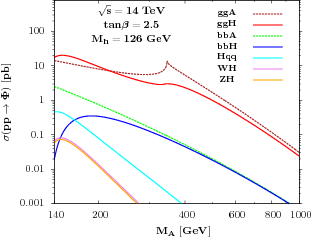
\includegraphics[scale=0.61]{fig/chapt2/Heavy_higgs_prod_xsec.png}
& \hspace{-0.3cm} 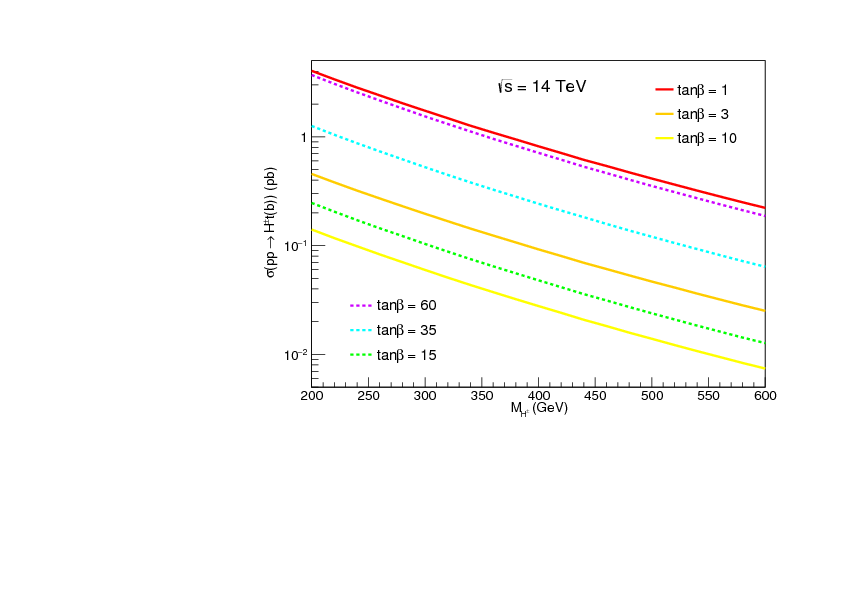
\includegraphics[trim={8cm 6.0cm 0 0},clip, scale=0.4]{fig/chapt2/plots_xs_Htb_14TeV.png}\\
  \qquad\qquad\qquad\qquad ($\mathbf{a}$)\qquad\qquad\qquad&($\mathbf{b}$)\\
\end{tabular}
\caption{(a): Heavy Higgs (neutral) boson production cross sections in MSSM for main channels with $\tan\beta$ = 2.5 and SM Higgs mass is 126 at $\sqrt{s} = 14 TeV$ w.r.t M$_{A}$. (b): Charged Higgs production cross sections for a range of $\tan\beta$ values w.r.t to M$_{H^{\pm}}$ \cite{Djouadi:2013vqa,Djouadi:2015jea}. }\label{fig:Heavy_H_prod_xsec}
\end{figure}
\noindent\textbf{Neutral Higgs decay}: The decay of neutral Higgs ($\Phi$ = H/A) is dictated by $\tan\beta$ value in a similar pattern as in production because of coupling sensitivity to $\tan\beta$. In decoupling limits ($\sin\left(\alpha-\beta\right) = 1$), the couplings of $\mathcal{CP}$-even state ($\cos\alpha/\cos\beta$) \ref{tab:couplings} explicitly equal to $\tan\beta$. For high $\tan\beta \gtrsim 10$, the couplings to b-quark and tau lepton enhanced and it decays exclusively to a $b\bar{b}$ or $\tau^{+}\tau^{-}$ pairs with branching ratios BR($\Phi\rightarrow b\bar{b} \approx 90\%$) and BR($\Phi\rightarrow \tau^{+}\tau^{-} \approx 10\%$) respectively. Decay to $t\bar{t}$ pair is highly suppressed for high $\tan\beta$ range as g$_{\Phi t\bar{t}} \propto 1/\tan\beta$. Other decay modes of $\mathcal{CP}$-even state H like in di-boson ($H\rightarrow VV; V= WW, ZZ$) and decay of $\mathcal{CP}$-odd state into lighter Higgs and Z bosons are strongly suppressed in the alignment limit approximation. For $H\rightarrow hh$ in the limit $M_{H}\gtrsim 2M_{h}$, the coupling $g_{Hhh}$ vanished at high $\tan\beta$ \cite{Baglio:2015wcg} 
\begin{equation}
g_{Hhh} = 2\sin2\alpha \sin\left(\alpha+\beta\right)-\cos2\alpha\cos\left(\alpha+\beta\right)+3\frac{\Delta M^{2}_{22}}{M^{2}_{Z}}\frac{\sin\alpha}{\sin\beta}\cos\alpha^{2}
\end{equation}
becomes
\begin{equation}
\begin{split}
g_{Hhh} \xrightarrow{\text{M}_{A}\gg \text{M}_{z}} -3\Delta \frac{M^{2}_{22}}{M_{Z}^{2}}\times \sin2\beta\\
\sin2\beta \propto \cot\beta \xrightarrow{\tan\beta \gtrsim 10} 0
\end{split} 
\end{equation}  
For $\Phi\rightarrow \gamma\gamma$ channel, the coupling is very small and shows a constant behaviour for $0.3\lesssim \tan\beta \lesssim 10$ which reduces abruptly for $\tan\beta \gtrsim 10$. Same pattern is followed by $\Phi \rightarrow gg$ channel but higher coupling compare to $\Phi\rightarrow \gamma\gamma$. For intermediate values of $\tan\beta \approx 5-10$ with M$_{\Phi} < 2m_{t}$, the bosonic decay of $H\rightarrow WW, ZZ$ has significant contribution as it's competition is only with the $H\rightarrow b\bar{b}$ decay. In this limit the $H\rightarrow t\bar{t}$ decay is suppressed as the phase-space is not feasible. At $\tan\beta$ = 2.5 and $2M_{h} \lesssim M_{\Phi}< 2m_{t}$, $H\rightarrow hh$ and $A\rightarrow hZ$ have prominent branching ratios. Figure \ref{fig:Heavy_H750_BR} shows branching ratios w.r.t $\tan\beta$ for a specific M$_{\Phi}$ = 750 GeV. Figure \ref{fig:Heavy_Hpm_BR}a and b show mass versus branching ratios for $\mathcal{CP}$-odd and $\mathcal{CP}$-even states for $\tan\beta$ = 2.5 and M$_{h}$ = 126 GeV. 
\begin{figure}[htp]
\centering
\hspace{-0.3cm} 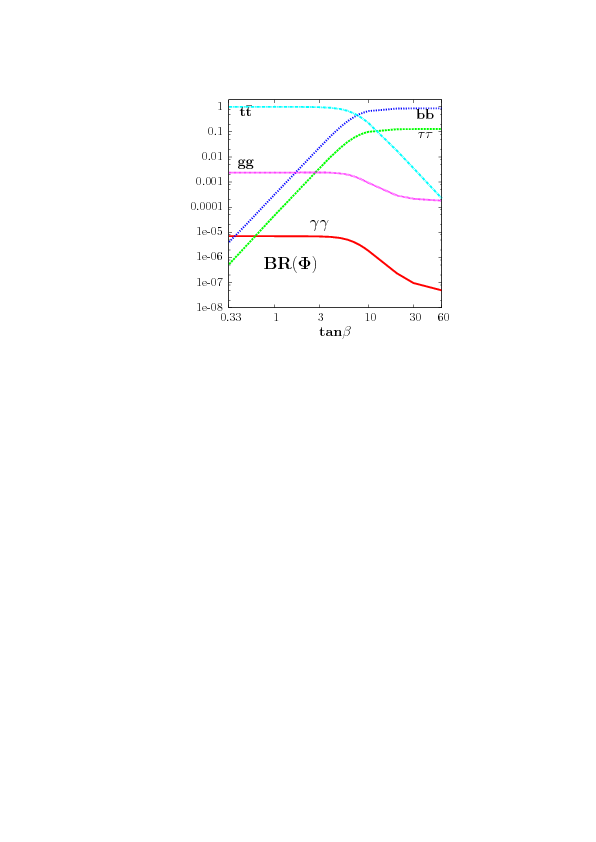
\includegraphics[trim={6cm 17.50cm 4.0cm 3.50cm},clip, scale=0.8]{fig/chapt2/BR-Atb.png}
\caption{The branching ratios of $\Phi$ = H/A in different channels as a function of $\tan\beta$ exploiting the M$_{\Phi}$ = 750 GeV \cite{Djouadi:2016eyy}. }\label{fig:Heavy_H750_BR}
\end{figure}
\\
\noindent \textbf{Charged Higgs decay}:
In high range of $\tan\beta \gtrsim 10$ with M$_{H^{\pm}} \lesssim m_{t} - m_{b}$, the dominant decay of H$^{\pm}$ occurs in the $H^{\pm}\rightarrow \tau\nu$ channel with a small fraction in hadronic decay mode. For high mass range,  M$_{H^{\pm}} > m_{t} - m_{b}$, the decay channel M$_{H^{\pm}} \rightarrow tb$ becomes the dominant one while $H^{\pm}\rightarrow \tau\nu$ branching ratio suppressed. A same saw pattern for the mentioned mass range is followed for low $\tan\beta$ by these two channels but this time the $H^{\pm}\rightarrow \tau\nu$ channel suppressed more compare to high $\tan\beta$. For low $\tan\beta$ and M$_{H^{\pm}} \gtrsim 160 $ GeV, another important channel, $H^{\pm}\rightarrow hW^{\pm}$, comes into play with smaller branching ratio than the $H^{\pm}\rightarrow tb$ one. Figure \ref{fig:Heavy_Hpm_BR}c shows branching ratios at a function of M$_{H^{\pm}}$ for H$^{\pm}$ at $\tan\beta$ = 2.5. Until now I discussed all the main decay channels for neutral and charged heavy higgs in different $\tan\beta$ ranges but there are many more with small contributions. To complete the picture, I write all of them in the form of total decay width equations. The total decay widths of neutral and charged Higgs are given in \ref{equ:neutral_decay_widths} and \ref{equ:charged_decay_widths} respectively. For completeness I mentioned the SUSY decay widths in the formulae. FH is abbreviation for $\mathtt{FEYNHIGGS}$ and HD stands for $\mathtt{HDECAY}$ programs commonly used for decay widths and branching ratio calculation of the Higgs boson with more detail is given here \cite{Dittmaier:2012vm}.
\begin{equation}\label{equ:neutral_decay_widths}
\begin{split}
\Gamma_{\Phi} = \Gamma^{\text{FH}}_{\Phi \rightarrow\tau^{+}\tau^{-}} + \Gamma^{\text{FH}}_{\Phi \rightarrow\mu^{+}\mu^{-}} + \Gamma^{\text{FH/P4f}}_{\Phi \rightarrow \text{W}^{*}\text{W}^{*}} + \Gamma^{\text{FH/P4f}}_{\Phi \rightarrow \text{Z}^{*}\text{Z}^{*}}\\
+ \Gamma^{\text{HD}}_{\Phi \rightarrow b\bar{b}} + \Gamma^{\text{HD}}_{\Phi \rightarrow t\bar{t}} + \Gamma^{\text{HD}}_{\Phi \rightarrow c\bar{c}} + \Gamma^{\text{HD}}_{\Phi \rightarrow gg} + \Gamma^{\text{HD}}_{\Phi \rightarrow \gamma \gamma} + \Gamma^{\text{HD}}_{\Phi \rightarrow \text{Z} \gamma}\\
+ \Gamma^{\text{FH}}_{\Phi \rightarrow \text{Zh}} + \Gamma^{\text{FH}}_{\Phi \rightarrow \text{hh}} + \Gamma^{\text{FH}}_{\Phi \rightarrow \text{ZA}} + \Gamma^{\text{FH}}_{\Phi \rightarrow \text{AA}}  + \Gamma^{\text{HD}}_{\Phi \rightarrow \text{H}^{\pm}\text{W}^{\mp}} + \Gamma^{\text{FH}}_{\Phi \rightarrow \text{SUSY}}
\end{split}
\end{equation}
\begin{equation}\label{equ:charged_decay_widths}
\begin{split}
\Gamma_{\text{H}^{\pm}} = \Gamma^{\text{FH}}_{\text{H}^{\pm} \rightarrow\tau\nu_{\tau}} + \Gamma^{\text{FH}}_{\text{H}^{\pm} \rightarrow\mu\nu_{\mu}} + \Gamma^{\text{FH}}_{\text{H}^{\pm} \rightarrow \text{hW}} + \Gamma^{\text{FH}}_{\text{H}^{\pm} \rightarrow \text{HW}} + \Gamma^{\text{FH}}_{\text{H}^{\pm} \rightarrow \text{AW}}\\
+ \Gamma^{\text{HD}}_{\text{H}^{\pm} \rightarrow \text{tb}} + \Gamma^{\text{HD}}_{\text{H}^{\pm} \rightarrow \text{ts}} + \Gamma^{\text{HD}}_{\text{H}^{\pm} \rightarrow \text{td}} +  \Gamma^{\text{HD}}_{\text{H}^{\pm} \rightarrow \text{cb}} + \Gamma^{\text{HD}}_{\text{H}^{\pm} \rightarrow \text{cs}} + \Gamma^{\text{HD}}_{\text{H}^{\pm} \rightarrow \text{cd}}\\
+ \Gamma^{\text{HD}}_{\text{H}^{\pm} \rightarrow \text{ub}} + \Gamma^{\text{HD}}_{\text{H}^{\pm} \rightarrow \text{us}} + \Gamma^{\text{HD}}_{\text{H}^{\pm} \rightarrow \text{ud}} + \Gamma^{\text{HD}}_{\text{H}^{\pm} \rightarrow \text{SUSY}}
\end{split}
\end{equation}
\begin{figure}[htp]
\centering
\begin{tabular}{ccc}
\hspace{-0.7cm}
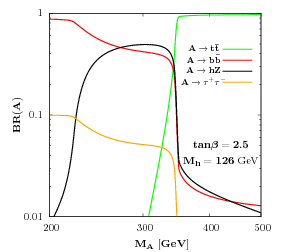
\includegraphics[scale=0.47]{fig/chapt2/A_br.png}
& \hspace{-0.65cm} 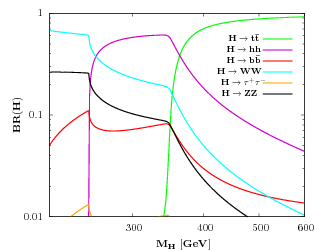
\includegraphics[scale=0.47]{fig/chapt2/H_br.png}
& \hspace{-0.65cm} 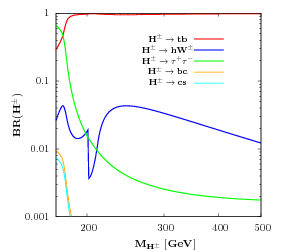
\includegraphics[scale=0.47]{fig/chapt2/H_pm_br.png}\\
  \qquad ($\mathbf{a}$)\qquad\qquad&($\mathbf{b}$)\qquad\qquad&($\mathbf{c}$)\\
\end{tabular}
\caption{Heavy Higgs decay branching ratios in MSSM, (a) pseudo scalar Higgs A, (b) Scalar Higgs H and (c) charged Higgs (H$^{\pm}$) with $\tan\beta$ = 2.5 and SM Higgs mass is 126. Plot are taken from \cite{Djouadi:2013vqa}. }\label{fig:Heavy_Hpm_BR}
\end{figure}
\noindent \subsection{The $\Phi \rightarrow t\bar{t}$ channel with interference from SM $gg \rightarrow t\bar{t}$}
\textbf{Introduction to interference:} In particle physics a process is represented by one or more Feynman diagrams and the resultant amplitude is expressed in terms of matrix element. For a given process, interference is the contribution from the cross terms of different processes to the final amplitude which introduces a peak, dip, nothingness or more complex peak-dip or dip-peak structure. It can be considered a similar phenomenon as quantum wave interference. Interference depends on physics model and it effects different kinematics of the searched particle in different ways. Most of particles discoveries are carried out by simply confirming a resonant peak in the transverse invariant mass distribution above the continuum backgrounds, like $J/\Psi$ meson, $W/Z$ bosons, higgs ($h$) boson and top quark. Currently most of LHC new physics searches focus on the same search strategy by looking to the access above the continuum background. But in some cases the kinematics (mass, $p_{T}$) of the searching particle are not pure Breit-Wigner (BW) resonance peak but instead a modified shape from the interfering background or other resonance. The complicated dip-peak or peak-dip structure is more sensitive to new physics than the simple resonant peak. It was first realised in the $gg\rightarrow\Phi\rightarrow t\bar{t}$ channel \cite{Gaemers:1984}. This channel along with interference effect is studied in this thesis and will be explained in detail after the general introduction to the interference. \\
\noindent Consider a two body scattering $ab\rightarrow {cd}$ whose partonic differential cross section w.r.t angular variable $z\cos\theta^{*}$, where $\theta^{*}$ is the scattering angle in the c.o.m frame, can be expressed as \cite{Jung:2015gta}   
\begin{equation}\label{equ:gen_interference}
\frac{d\hat{\sigma}}{dz}=\frac{1}{32\pi\hat{s}}\sum \left| \mathcal{A}_{\text{bg}}e^{i\phi_{\text{bg}}}+\frac{M^{2}}{\hat{s}-M^{2}+iM\Gamma}.\mathcal{A}_{\text{res}}e^{i\phi_{\text{res}}} \right|^{2}.
\end{equation}
In equation \ref{equ:gen_interference} the sum is for all spin and color components, $\hat{s}$ is the partonic energy and $\phi_{bg,res}$ is the complex phase of background and resonant part respectively. $\mathcal{A}_{bg}$ shows the continuum background amplitude and the term $\mathcal{A}_{res}$ is resonance amplitude for the searching particle with mass A and width $\Gamma$. Expanding the square and re-arranging, we get equation \ref{equ:split_inter} where we define new terms, $\sigma_{int}$, R, $\omega$ and $\phi = \phi_{res}-\phi_{bg}$ with definitions in equation \ref{equ:inter_variables}.  

\begin{equation}\label{equ:split_inter}
\hat{\sigma}=\hat{\sigma}_{\text{bg}}+\frac{M^{4}}{\left(\hat{s}-M^{2}\right)^{2}+M^{4}\omega^{2}}\times\left[\frac{2\left(\hat{s}-M^{2}\right)}{M^{2}}\hat{\sigma}_{\text{int}}c_{\phi}+\hat{\sigma}_{\text{res}}\left(1+\frac{2\omega}{R}s_{\phi} \right) \right]
\end{equation}
where c$_{\phi}$ = cosine$\phi$ and s$_{\phi}$ = sine$\phi$.
\begin{equation}\label{equ:inter_variables}
\begin{split}
\hat{\sigma}_{\text{bg,res}}=\frac{1}{32\pi\hat{s}}\int dz \sum \mathcal{A}^{2}_{\text{bg,res}},\\
\hat{\sigma}_{\text{int}}e^{i\phi}=\frac{1}{32\pi\hat{s}}\int dz \sum \mathcal{A}_{\text{bg}}\mathcal{A}_{\text{res}}e^{i\left(\phi_{\text{res}}-\phi_{\text{bg}}\right)},\\
R=\frac{\hat{\sigma}_{\text{res}}}{\hat{\sigma}_{\text{int}}},\qquad \omega \equiv \frac{\Gamma}{M}.
\end{split}
\end{equation}
\noindent $\omega$, R and  $\phi$ are parameters of interest with the later two are respectively relative strength and phase difference between signal resonance and background continuum. The second interference term in equation \ref{equ:split_inter} further consists of two parts, the real with $\text{c}_{\phi}$ and imaginary s$_{\phi}$, decides the final interference pattern. The well known peak-dip or dip-peak structure arises from the real interference part with s$_{\phi}$ = 0 with a final shift in the resonance peak position. We are focusing on the pure resonance as well as peak-dip structure of the signal in this analysis. The imaginary term makes the shape more interesting at specific conditions of $\phi$ and factor C where C is defined as
\begin{equation}\label{equ:correction_term}
C \equiv \left(1+\frac{2\omega}{R}s_{\phi} \right).
\end{equation} 
At $\phi=-\pi /2$ and C < 0, the $gg\rightarrow\Phi\rightarrow AB$ line adopted a pure dip shape shown in figure \ref{fig:dip_peak_nothing_H_A}a by the green line. On contrary, the access can be achieved by C > 0 shown by the orange line in figure \ref{fig:dip_peak_nothing_H_A}a where its amplitude can be increased or decreased relative to pure resonance (dashed-orange line) by varying the value of $\phi$. At $\phi=-\pi /2$ and C = 0, the line shape becomes more interesting when both the real and imaginary part disappear and the signal line now running parallel with continuum background. These types of shapes are termed as "nothingness" and need more careful treatment. All the above defined signal structures demand a new search strategy compare to what we are searching for simple resonance. 

\begin{figure}[htp]
\centering
\begin{tabular}{cc}
\hspace{-0.3cm}
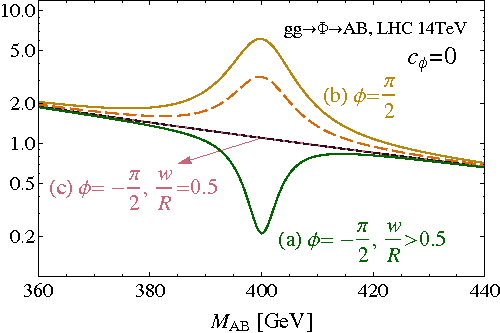
\includegraphics[scale=0.41]{fig/chapt2/dip_peak_nothing.png}
& \hspace{-0.45cm} 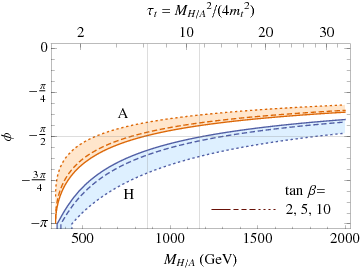
\includegraphics[scale=0.61]{fig/chapt2/fig_phase_A_H.png}\\
  \qquad\qquad\qquad ($\mathbf{a}$)\qquad\qquad\qquad\qquad&($\mathbf{b}$) \\
\end{tabular}
\caption{(a): Resonance shapes after pure imaginary interference (c$_{\phi}$ = 0) with mass = 400 GeV, $\Gamma$ = 10 GeV and R = 0.035. Green line is pure dip, orange is access, orange-dashed is pure resonance, red is nothingness and solid black is continuum background. Arbirary units are used on y-axis. (b): shows the relative phase $\phi$ between continuum $gg\rightarrow t\bar{t}$ and resonace $gg\rightarrow \Phi \rightarrow t\bar{t}$ w.r.t M$_{H/A}$ at different $tan\beta$ values (2, 5, 10) with $\tau_{t} = M^{2}_{H/A}/(4m_{t}^{2})$ at the upper horizental axis. For all values of $tan\beta$, the $-\pi/2$ condition achieved by $\mathcal{CP}-$odd state ($A$) much faster than the $\mathcal{CP}-$even state ($H$) shown by vertical lines \cite{Jung:2015gta}. }\label{fig:dip_peak_nothing_H_A}
\end{figure}

\begin{figure}[htp]
\centering
\begin{tabular}{cc}
\hspace{-0.3cm}
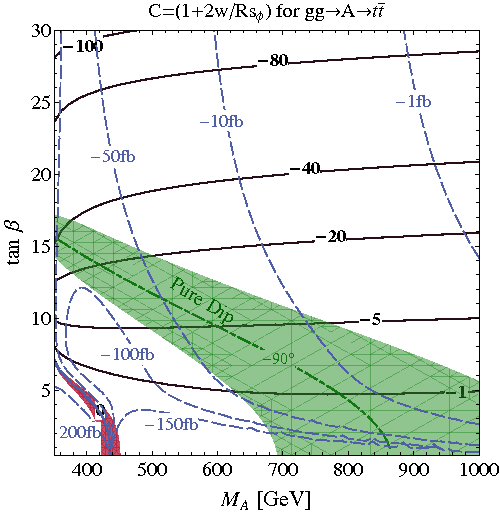
\includegraphics[scale=0.42]{fig/chapt2/nwafix-ttbar-A.png}
& \hspace{-0.4cm} 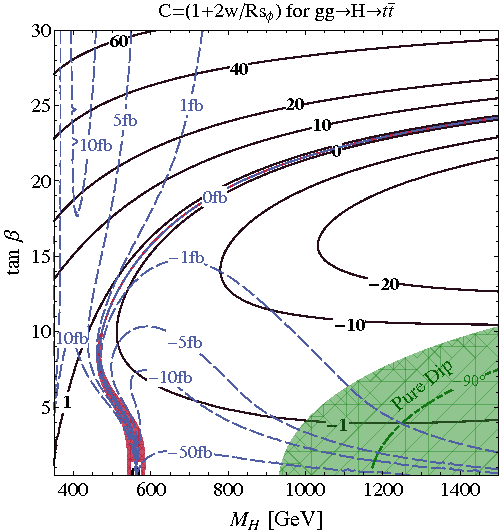
\includegraphics[scale=0.4]{fig/chapt2/nwafix-ttbar-H.png}\\
  \qquad ($\mathbf{a}$)\qquad\qquad&($\mathbf{b}$) \\
\end{tabular}
\caption{ \cite{}. }\label{fig:NWA_H_A}
\end{figure}


The correlation resulting from projecting the spin of $t$ onto the spin of \cite{Berge:2008dr, PhysRevD.58.114031}
\begin{equation}
\left\langle S \right\rangle = \frac{a_{1}^{2}-3a_{2}^{2}}{4a_{1}^{2}+4a_{2}^{2}}
\end{equation}\label{equ:tt_spin}
\begin{figure}[htbp]
\centering
%\hspace{2.0cm}
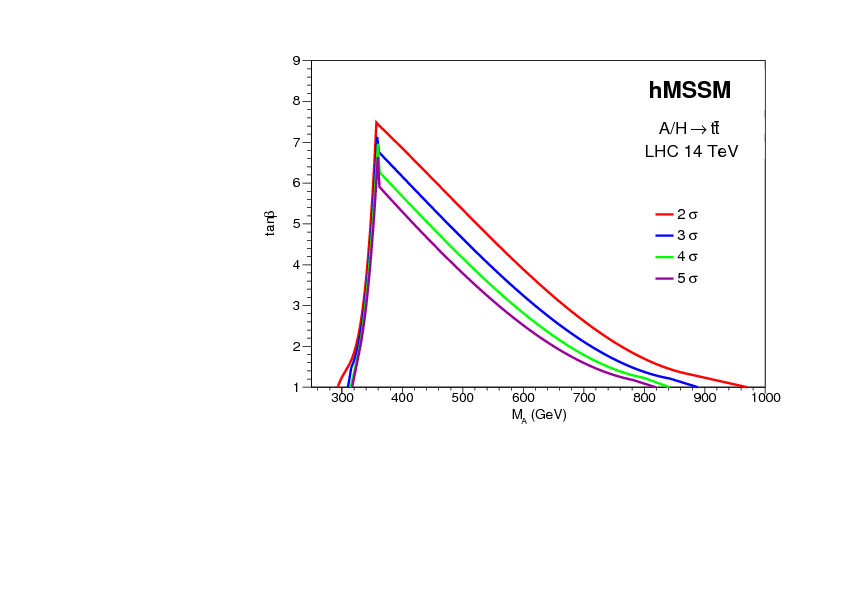
\includegraphics[trim={8cm 6.0cm 0 0},clip, scale=0.6]{fig/chapt2/plots_constraints_LHC14_300_AH_tt.png}
\caption{Sensitivity levels for $\Phi\rightarrow t\bar{t}$ channel at $\sqrt{s}=14$ TeV with total integrated luminosity $\mathcal{L}=300 \text{f}\text{b}^{-1}$ in hMSSM and ($\tan\beta, \text{M}_{A}$) plane. At M$_{\Phi} \approx 2\text{m}_{t}$, we have a large $\tan\beta$ space upto 7.5 which shows the sensitivity of the top quark to new physics \cite{Djouadi:2015jea}. }\label{fig:Htt_sensitivity}
\end{figure}


\begin{figure}[htp]
\centering
\begin{tabular}{cc}
\hspace{-0.3cm}
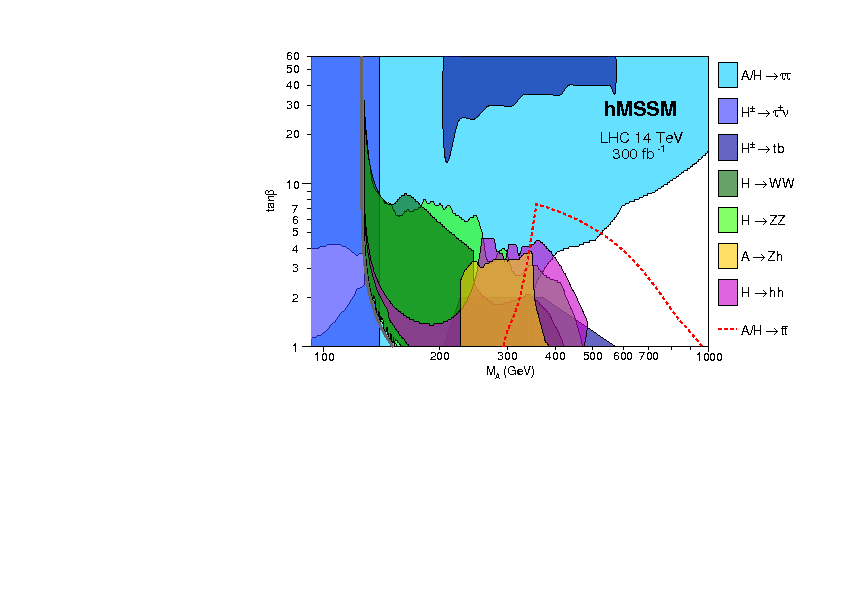
\includegraphics[trim={8cm 6.0cm 0 0},clip, scale=0.4]{fig/chapt2/httplots_constraints_LHC14_300fb_all.png}
& \hspace{-2.4cm} 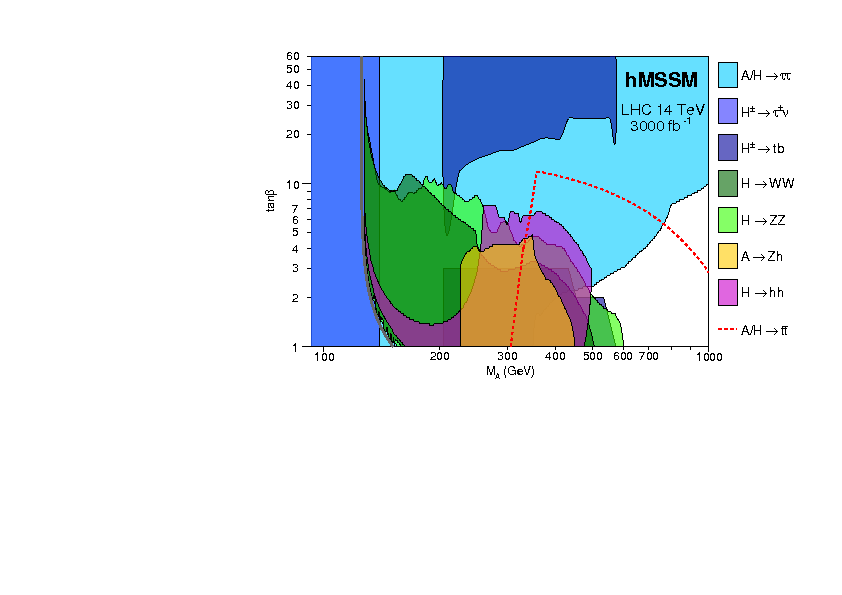
\includegraphics[trim={8cm 6.0cm 0 0},clip, scale=0.4]{fig/chapt2/httplots_constraints_LHC14_3000fb_all.png}\\
  \qquad ($\mathbf{a}$)\qquad\qquad&($\mathbf{b}$)\qquad\qquad\qquad\qquad \\
\end{tabular}
\caption{All decay channels of neutral and charged Higgs with expectation of 2$\sigma$ at $\sqrt{s}=14$ TeV using hMSSM with total integrated luminosity $\mathcal{L}=300 \text{f}\text{b}^{-1}$ (a) and  HL-LHC $\mathcal{L}=3000 \text{f}\text{b}^{-1}$ (b) using hMSSM and ($\tan\beta, \text{M}_{A}$) plane. The red-dashed contour shows the $\Phi\rightarrow t\bar{t}$ channel where it's sensitivity lies in low $\tan\beta$ and high mass region \cite{Djouadi:2015jea}. }\label{fig:Heavy}
\end{figure}
   
\clearpage{\pagestyle{empty}\cleardoublepage}
